\documentclass[letterpaper,onside,11pt]{book}

\usepackage[paperwidth=17cm, paperheight=22.5cm, bottom=2.5cm, right=2.5cm]{geometry}
\usepackage[utf8]{inputenc}
\usepackage[spanish]{babel}
\usepackage{algorithm}
\usepackage{amsmath}
\usepackage{amssymb}
\usepackage{amsthm}
\usepackage{hyperref}
\usepackage{graphicx}
\usepackage{subfig}
\usepackage[toc,page]{appendix}
 
\usepackage[round]{natbib}
%\bibliographystyle{apalike}
%\bibliographystyle{chicago}
\bibliographystyle{unsrtnat}
 
\title{Inferencia Bayesiana en Modelos de Mezcla en Media-Marianza}
\author{David Edgardo Castillo Rodr\'iguez}
\date{\today}
 
%	Commands
\renewcommand{\chaptername}{Cap\'itulo}
\renewcommand{\figurename}{Gr\'afica}
\usepackage{setspace}
%\singlespacing        %% 1-spacing (default)
\onehalfspacing       %% 1,5-spacing
%\doublespacing        %% 2-spacing
\pagestyle{plain}

%
%	Documento
%
\begin{document}
 
%	Title
%\maketitle	% comenta esta instruccion para la version final

\begin{titlepage}
	\begin{center}
		
		\textsc{\Large Instituto Tecnol\'ogico Aut\'onomo de M\'exico}\\[4em]
		
		%Figura
		\begin{center}
			
\includegraphics{DocumentosLaTex/ITAM_2016.png}
		\end{center}
		
		\vspace{2em}
		
		{\sc \huge {\bf Inferencia Bayesiana en Modelos de Mezcla en Media-Marianza}}\\[4em]
		
		\textsc{\large Tesis}\\[1em]
		
		\textsc{que para obtener el t\'itulo}\\[1em]
		
		\textsc{Licenciado en Actuar\'ia}\\[1em]
		
		\textsc{presenta}\\[1em]
		
		\textsc{\Large David Edgardo Castillo Rodr\'iguez}\\[1em]
		
		\textsc{\large Asesor: Juan Carlos Mart\'inez Ovando}
		
	\end{center}
	
	\vspace*{\fill}
	\textsc{Ciudad de M\'exico \hspace*{\fill} 2017}
	
\end{titlepage}

%	
\tableofcontents

% Capitulos
\chapter{Introducción}

Con el fin de modelar algún fenómeno de interés de la natraleza se han propuesto modelos estocásticos, como la selección de un portafolio de mínima varianza, o la segmentación de individuos mediante un análisis de discriminante, por ejemplo. Estos modelos estocásticos suponen que los datos tienen alguna estructura de correlación dada, como es el caso del portafolio de mínima varianza que presupone una estructura de correlación normal; otros modelos requieren la estimación de alguna ley de probabilida, donde muchas veces se utiliza la distribución normal (o una mezcla finita normal), por su practicidad.   

Dicho lo anterior, la presente tesis fue motivada por la siguiente pregunta ¿Qué hacer cuando hay evidencia de que un conjunto de datos no sigue una ley de probabilidad normal? Varios investigadores han dado respuesta a esta pregunta, mediante la distribución $T$, o la incorporación de un sesgo a la distribución normal (o a la distribución $T$), o mediante el uso de cópulas, o mediante el uso de la distribución hiperbólica generalizada, por ejemplo. De aquí que el tema central de esta tesis sea el cómo estimar una distribución hiperbólica (caso particular de la distribución hiperbólica generalizada).

El problema de cómo ajustar una distribución hiperbólica se realizará mediante distribuciones tipo mezcla normal en esperanza y varianza, ya que está distribución permite simplificar el problema, también para realizar el ajuste se utilizará un enfoque bayesiano, ya que se adecua de manera natural a las distribuciones tipo mezcla normal, y además permite explotar el conocimiento a priori de los datos para la obtención de los parámetros de la distribución a estimar.

La presente tesis se divide un $6$ capítulos. En el capítulo $1$ se introduce de manera breve el paradigma bayesiano de inferencia, el cual es necesario para el tipo de estimación que se hará. En el capítulo $2$ se expone la notación a usar, así como las distribuciones necesarias para la estimación; también se habla brevemente de algunas características de las distribuciones mencionadas. En el capítulo $3$ se introducen las distribuciones tipo mezcla normal, para así poder caracterízar a la distribución hiperbólica; también se habla brevemente de algunas características de estas distribuciones. En el capítulo $4$ se construyen la función de verosimilitud, y densidades marginales completas necesarias para la estimación. En el capítulo $5$ se hablará de los resultados y conclusiones. Y por último, en el capítulo $6$ se incluye como anexo algunos resultados utilizados utilizados en la presente tesis, así como los respectivos códigos implementados, es importante mencionar que para la obtención de resultados se utilizó el software $R$.


 
\chapter{Introducción al paradigma bayesiano de inferencia} 
En este capítulo se hablará brevemente sobre los antecedentes del paradigma bayesiano de inferencia, así como de algunas ideas principales que dieron
origen a este. Y así, concluir en cómo es la estimación bayesiana, la cual es fundamental en este trabajo.

\section{Antecedentes}

En 1763, dos años después de la muerte de Thomas Bayes $(1702-1761)$, se publicó uno de sus ensayos, el cual consistió en resolver un problema de información inversa planteado por Jacob Bernoulli (An Essay towards solving a Problem in the Doctrine
of Chances). El problema de Bernoulli consitia en obtener información sobre la realización de variables aleatorias independientes distribuidas Bernoulli; para ello, Bayes propuso en su ensayo un método que consistia en tener una suposición sobre la posibilidad de que un evento que tenga que ocurrir, algunas veces ocurra con éxito y otras veces no ocurra (o sea, un fracaso).

En este punto de la historia, las ideas de Bayes carecian de claridad, pero diez años más tarde se esclarecieron debido a que Laplace las retomó, dandole así forma al paradigma Bayesiano de inferencia. Dichas ideas se consolidaron en su libro Theoriè analytique des probabilitès, 1812. Pero el trabajo de Laplace (concerniente al paradigma Bayesiano) aún carecia de formalidad teórica.

El paradigma bayesiano de inferencia cuntinuó eclipsado, hasta que Harold Jeffrey (Theory of probability, 1939), y Bruno De Finetti (La Prévision, ses Lois Logiques, ses Sources Subjectives, 1937) desarrollaron y dieron sustento teórico al paradigma bayesiano. Harold Jeffrey mantuvo una postura objetiva dentro del paradigma bayesiano, ya que el decía que la información inicial era capturada objetivamente mediante el uso de distribuciones no informativas. Por otro lado, De Finetti mantuvo una postura subjetiva, ya que en su obra se desarrolla la teoría de probabilidad refiriendose a esta como un grado un grado de creencia.

Hasta la fecha, el paradigma bayesiano sigue introduciendose en distintos campos de la ciencia, ya que es una gran herramienta en de inferencia o predicción, lo cuál es de vital interés en ciertos ámbitos de la vida humana, como en finanzas, econometría, actuaría, por ejemplo (en Savage (1972) o Lindley (1957) se puede encontrar una explicación más profunda del paradigma bayesiano de inferencia). 

Ahora, teniendo un contexto sobre la evolución del paradigma bayesiano, veamos cuales son sus principios técnicos, y la idea que hay en estos.

\section{Proceso de aprendizaje}  

Supongamos que tenemos un conjunto de eventos $A_{1}$, $A_{2}$, . . ., $A_{n}$, de los cuales nos gustaría hacer inferencia de acuerdo a una función de probabilidad, $P$, (referente a estos eventos), y con un nivel de información o evidencia disponible, el culal denotaremps por $B$. Con estos elementos podemos definir nuestro estado de información actual sobre los eventos $A_{1}$, $A_{2}$, . . ., $A_{n}$, dada nuestra información inicial $B$, lo cual queda expresado, para cualquier $A_{i}$, como: $P(A_{i}|B)$, donde $\sum_{i=1}^{n}A_{i}=1$.

Ahora, lo que nos interesa es actualizar nuestro nivel de información actual dada nueva información, digamos $C$, lo cual lo conseguimos de la siguiente manera utilizando la definición de probabilidad condicional \cite{Ross_Book},
\begin{eqnarray}
	P(A_{i}|C \wedge B)&=&\frac{P(A_{i} \wedge C \wedge B)}{P(C \wedge B)} \nonumber \\
	&=& \frac{P(A_{i} \wedge B)}{P(B)} \frac{P(B)}{P(C \wedge B)} \frac{P(C \wedge A_{i} \wedge B)}{P(A_{i} \wedge B)} \nonumber\\
	&=& P(A_{i}|B)P(C | A_{i} \wedge B)/P(C | B) \nonumber\\
\end{eqnarray} 

La ecuación anterior representa la idea de proceso de aprendizaje, o sea, dado el nivel de evidencia inicial denotado por $B$, mediante la incorporación de nueva información donotada por $C$, podemos actualizar nuestras creencias que ya teniamos con respecto al evento $A_{i}$, es decir, pasar de solamente tener $P(A_{i}|B)$ a $P(A_{i}|B \wedge C)$.

\section{El proceso de aprendizaje en la inferencia estadística}

Aplicando las ideas de la sección anterior, podemos incorporar nueva información en una distribución de probabilidad paramétrizada, cuyo parámetro es desconocido para nosotros. Este desconocimiento del verdadero valor del parámetro lo incorporamos en un distribución de probabilidad propia del parámetro desconocido. Por notación nos referimos a la distribución de probabilidad del parámetro como distribución inicial, y la denotamos como : $\Pi(\theta)$, donde $\theta$ es el parámetro descocnocido el cual pertenece a un espacio parametral $\Theta$.

Dicho lo anterior, dada una variable aleatoria $X$ con distribución de densidad de probabilidad parametrizada por algún parámetro $\theta$, tenemos la distribución $f_{X}(x|\theta)$ la cual se lee como distribución de $X$ dado $\theta$. Después, incorporando nuestro desconocimiento de $\theta$, con $\Pi(\theta)$ podemos formular la siguiente expresión:

\begin{eqnarray}
	\Pi(\theta|X)&=&\frac{f(x \wedge \theta)}{f(x)}\nonumber\\
	&=&\frac{f(x \wedge \theta)}{f(x)} \frac{\Pi(\theta)}{\Pi(\theta)}\nonumber\\
	&=&f(x|\theta)\frac{\Pi(\theta)}{f(X)}
\end{eqnarray}

De la ecuación $(2.2)$ podemos tener la siguiente expresión $\Pi(\theta|X) \propto f(x|\theta)\Pi (\theta)$. La parte derecha de la expresión anterior se conoce como distribución a posteriori de $\theta$, esta se puede interpretar como la actualización del nivel de información que teniamos de $\theta$ (dicho nivel de información está considerado en $\Pi(\theta)$), al incluir nueva información proveniente de la realización (o realizaciones) de la variable aleatoria $X$. 

La información proveniente de la variable aleatoria $X$ queda capturada por su función de densiadad condicionada por $\theta$, es decir, $f(x|\theta)$; también a esta densiadad condicionada la conocemos como función de verosimilitud.El símbolo $\propto$ nos indica que la expresión de la izquierda es proporcional a la de la derecha, es decir, sólo difieren por una constante que no depende del argumento de la parte izquierda.

La expresión $(2.2)$ también nos da un algoritmo recursivo, el cual nos permite mejorar nuestra información del parámetro $\theta$ conforme más información obtengamos de la variable aleatoria $X$, es decir, si consideramos una nueva ralización de $X=x*$, entonces nuestras nueva distribución apriori o inicial es $\Pi(\theta|x)$, mientras que la distribució a posteriori (o actualizada) queda dada como $\Pi(\theta|x \wedge x*)$, por lo que mediante un proceso análogo a $(2.2)$ tendriamos la siguiente expresión:
\begin{equation}
	\Pi(\theta|x \wedge x*)\propto f(x\wedge x*|\theta) \Pi(\theta|x \wedge x*)
\end{equation}

\section{Predicción}

Hasta ahora hemos visto cómo incorporar nueva información de la variable aleatoria $X$ para actualizar la información deisponible del parámetro $\theta$. Pero también podemos formularnos la siguientes preguntas ¿Qué pasa con el próximo valor de $X$ dados los valores $x$ que ya fueron observados? ¿Hay forma de que la infromación previa de $X$ sea incorporada para mejorar el nivel de información de futuras realizaciones? 
La respuesta a las preguntas anteriores tiene connotación positiva, y queda representada por la siguiente expresión:
\begin{eqnarray}
	f(y*|\overline{y})&=&\int_{S_{\theta}}f(y* \wedge \theta |\overline{y})d\theta\nonumber\\
	&=&\int_{S_{\theta}}f(y* | \theta \wedge \overline{y})\Pi(\theta) d\theta,
\end{eqnarray}  
donde $y*$ representa la realización futura de $Y$, $\overline{y}$ representa un conjunto de realizaciones
observadas de $Y$, y $\theta$ el parámetro de la distribución de probabilidad de $Y$.

\chapter{Preliminares}

En este capítulo se expone de manera breve la notación y algunas características de las distribuciones gaussiana, gaussiana $p$ variada, gamma, gamma inversa, Wishart, Wishart inversa, gaussiana inversa generalizada, gaussiana inversa, las cuales se usarán en capítulos posteriores.

La notación a emplear adoptará la usada en el enfoque bayesiano, para ser consistente
con el tipo de modelación que se realizará. Por lo que si la variable o vector aleatorio, $X$, tiene una función de densidad parametrizada por algún vector de parámetros, $\Theta$, entonces la función de densidad de $X$ se denotará por $f(X|\Theta)$, que se lee e interpreta como: $X$ se distribuye $f(x)$ dado $\Theta$. La función de densidad de $\Theta$ será $f(\Theta|\theta_{0})$ para algún vector de parámetros $\theta_{0}$. Esta función de densidad es conocida como distribución a priori, y se interpreta de la misma manera que la distribución de $X$, salvo que representa un grado subjetivo de creencia respecto a $\Theta$. Para la función de densidad de $\Theta$ condicionada en $X$ usaremos la notación $f(\Theta|X)$, la cual se conoce como densidad a posteriori (Bernardo $\&$ Smith, $2000$)\cite{}. 

\section{Distribución gaussiana}
Se dice que una variable aleatoria $X$, que toma valores en los números reales, se distribuye normal con media $\mu$, y desviación estándar $\sigma$, si su función de densidad de probabilidad es de la siguiente manera,

\begin{equation}
	f_{x}(x|\mu, \sigma)=\frac{1}{2\sqrt{\pi \sigma}}\exp^{-\frac{(x-\mu)^2}{2\sigma^2}}I_{(-\infty,\infty)}(x).
\end{equation}

En la distribución gaussiana, dos parámetros caracterizan la forma de la distribución,  $\mu=E[X]$, y $\sigma^2=Var[X]$, de aquí que el parámetro $\mu$ nos da información sobre la localización de la distribución, mientras que $\sigma$ de la dispersión.

Para referirnos a que $X$ se distribuye gaussiana con parámetros $\mu$ y $\sigma$, usaremos la notación, $X|\mu,\sigma$ se distribuye $N(x|\mu,\sigma)$.

Como se mencionó anteriormente, el parámetro $\mu$ es una medida de localización, mientras que el parámetro $\sigma$ es una medida de dispersión de la distribución gaussiana, lo cual se ilustra en las siguientes gráficas. En la gráfica \ref{fig:Ncambioenmedia} se pueden observar cuatro distribuciones gaussianas, etiquetadas como a), b), c) y d), con el mismo parámetro de dispersión $\sigma=1$, pero diferentes parámetros de localización, es decir,  $\mu_{1}=0$, $\mu_{2}=2$, $\mu_{3}=4$ y $\mu_{4}=6$ respectivamente.

\begin{figure}[h!]
	\centering
	%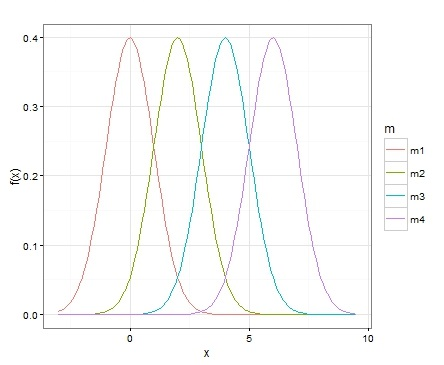
\includegraphics{Figuras/cambiosenmedia}
	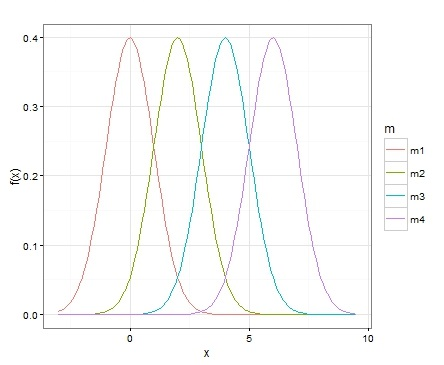
\includegraphics[width=.8\linewidth]{Figuras/cambiosenmedia.jpeg}
	\caption{Distribuciones gaussianas con el mismo par\'ametro de dispersi\'on, pero diferentes par\'ametros de localizaci\'on.}
	\label{fig:Ncambioenmedia}
\end{figure}

Por otro lado, en la gráfica \ref{fig:Ncambiosd}, se pueden observar cuatro distribuciones gaussianas, etiquetadas como a), b), c) y d), con parámetros de localización $\mu_{1}=0$, $\mu_{2}=0$, $\mu_{3}=0$ y $\mu_{4}=0$, y parámetros de dispersión $\sigma_{1}=0$, $\sigma_{2}=2$, $\sigma_{3}=4$ y $\sigma_{4}=6$, respectivamente; adviértase cómo incrementan las colas de la distribución gaussiana entre mayor es el parámetro de dispersión.

\begin{figure}[ht]
	\centering
	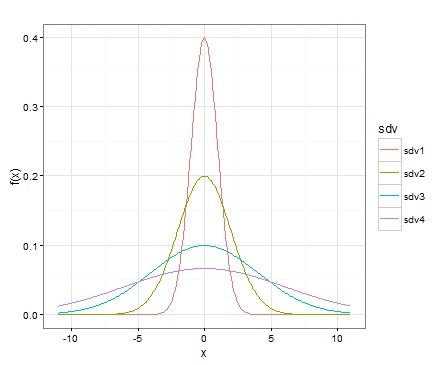
\includegraphics[width=.8\linewidth]{Figuras/cambiosd}
	\caption{Distribuciones gaussianas con diferente parámetro de dispersión.}
	\label{fig:Ncambiosd}
\end{figure}

\pagebreak

Como caso particular de la distribución gaussiana tenemos la distribución gaussiana estándar, que se obtiene cuando el parámetro $\mu =0$, y $\sigma=1$. También podemos llegar a esta distribución mediante un proceso de normalización de la distribución ($2.1$), es decir, si $X$ se distribuye  $N(x|\mu,\sigma)$, y si consideramos la transformación $Y=\frac{X-\mu}{\sigma}$, entonces $Y$ se distribuye $N(y|0,1)$.

Por último, la función generadora de momentos y característica de una distribución gaussiana es de la siguiente manera (Ross Shelder, Probability ),
\begin{equation}
	m_{x}(t)=\exp^{\sigma t+\frac{t\mu\sigma^2}{2}}
\end{equation}

\begin{equation}
	\Phi_{x}(it)=\exp \{\sigma it+\frac{it\mu\sigma^2}{2} \}
\end{equation}


\section{Distribución gaussiana p-variada}
Se dice que un vector aleatorio $X$ de dimensión $p$, con parámetros $\mu$ y $\Sigma$, que toma valores tanto positivos como negativos en cada entrada, tiene una distribución gaussiana $p$-variada  si su función de densidad es de la siguiente forma:
\begin{equation*}
	f_{x}(X|\mu,\Sigma)=\dfrac{1}{(2\Pi)^{p/2}|\Sigma|^{1/2}}exp\{-1/2(X-\mu)'\Sigma^{-1}(X-\mu)\}I_{R^{p}}(x),
\end{equation*}
donde $\mu=E[X]$, de dimensión $p$, es el vector de medias, y $\Sigma=Cov[X]$ de dimensión $p\times p$, matriz simétetrica positiva definida, es la matriz de varianza-covarianza. Análogamente a la distribución gaussiana, el vector $\mu$ es un vector de posición, el cual indica donde está centrada la distribución del vector aleatorio $X$. Mientras que la matriz $\Sigma$ está formada por las varianzas de cada $X_{i}$ en las entradas diagonales, es decir en la $(i,i)$ entrada, y por las covarianzas $Cov[X_{i,j}]$ en la $(i,j)$ entrada de la matriz. De aquí que la matriz de varianzas-covarianzas indique la dispersión del vector aleatorio $X$ alrededor del vector de medias $\mu$.

En este caso, si $X$ es un vector aleatorio de dimensión $p$, con vector de medias $\mu$, y matriz ve varianza-covarianza $\Sigma$, usaremos la notación $X$ se distribuye $N_{p}(x|\mu,\Sigma)$.

Como se mencionó anteriormente el vector $\mu$ es un parámetro de localización, de la distribución gaussiana $p$-variada, lo cual se ilustra a continuación para el caso bivariado. En la gráfica \ref{fig:NPM} se muestran  tres distribuciones gaussianas a), b) y c); todas con la misma matriz de varianza-covarianza $I$, con $\sigma_{1}=\sigma_{2}=1$ y $\sigma_{1,2}=0$; pero con vectores de medias $\mu_{1}=(-2,-2)$, $\mu_{2}=(0,0)$ y $\mu_{3}=(2,2)$, respectivamente. 

\begin{figure}[ht]
	\centering
	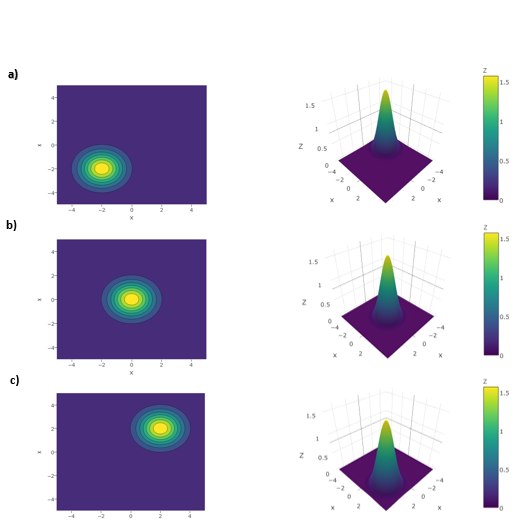
\includegraphics[width=.8\linewidth]{Figuras/NPM}
	\caption{Distribución gaussiana $p$-varaida con diferentes vectores de medias $\mu$.}
	\label{fig:NPM}
\end{figure}

\pagebreak
Ahora si nos enfocamos en la matriz de varianza-covarianza $\Sigma$, entre mayor sea la varianza del elemento $x_{i}$ del vector aleatorio $X$, mayor será la dispersión de la distribución de $X$ en el eje coordenado correspondiente a $x_{i}$.

Por otro lado, entre mayor o menor sea la covarianza entre algún par de elementos $x_{i}$ y $x_{j}$ pertenecientes a $X$, la distribución de $X$ tendrá una notable forma elíptica en los ejes cordenados $i$ y $j$, la cual está ligada a la interpretación de la correlación lineal entre $x_{i}$ y $x_{j}$, pues si $Cov[x_{i},x_{j}]$ es mayor a cero, la distribución de $X$ tendrá una foma elíptica centrada en el vector de medias $\mu$, pero rotada entre $0$ y $90$ grados, lo que indica que hay una dependencia lineal positiva entre el $i$-ésimo y $j$-ésimo elemento de $X$. Mientras que, sí la covarianza entre el $i$-ésimo y $j$-ésimo elemento de $X$ es menor a cero, la distribución de $X$ en los ejes coordenados $i$ y $j$ tendrá una forma elíptica rotada entre $90$ y $180$ grados. Los dos puntos anteriores se ilustran a cuntinuación para el caso bivariado.

En la gráfica \ref{fig:NPMsd} a) se observa una distribución gaussiana bivariada con vector de medias $\mu=(0,0)$, y con matriz de varianza-covarianza, $\Sigma$, con las entradas $Var[X]=1$, $Var[Y]=5$ y $Cov[X,Y]=0$. En b) con vector de medias $\mu=(0,0)$, $Var[X]=1$, $Var[Y]=1$ y $Cov[X,Y]=0$. Y en c) con vector de medias $\mu=(0,0)$, $Var[X]=5$, $Var[Y]=1$ y $Cov[X,Y]=0$. 

En la gráfica \ref{fig:NPcor} a) se observa una distribución gaussiana bivariada con vector de medias $\mu=(0,0)$, y con matriz de varianza-covarianza, $\Sigma$, con las entradas $Var[X]=2$, $Var[Y]=2$ y $Cov[X,Y]=0.75$. En b) con vector de medias $\mu=(0,0)$, $Var[X]=5$, $Var[Y]=5$ y $Cov[X,Y]=-0.75$. 

\begin{figure}[ht]
	\centering
	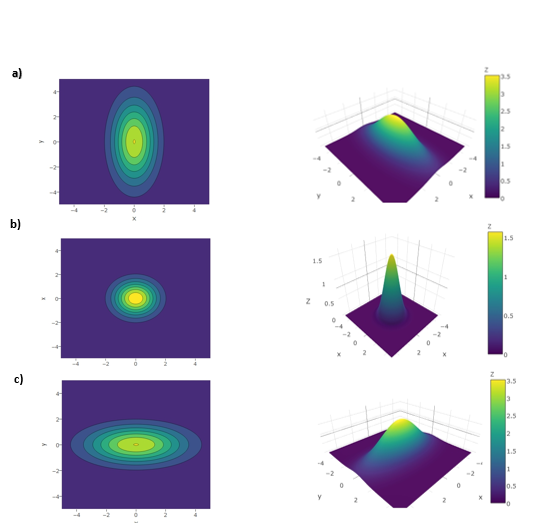
\includegraphics[width=.9\linewidth]{Figuras/NPMsd}
	\caption{Distribución gaussiana bivariada con diferentes varianzas y covarianzas}
	\label{fig:NPMsd}
\end{figure}

\begin{figure}[ht]
	\centering
	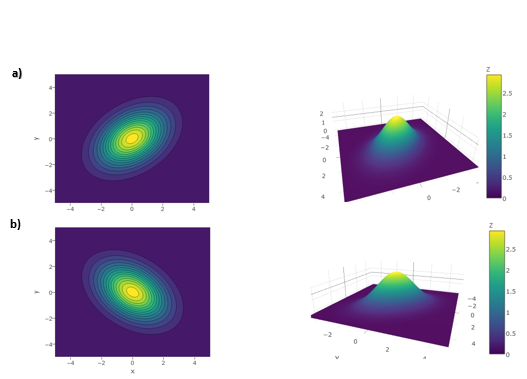
\includegraphics[width=.9\linewidth]{Figuras/NPcor}
	\caption{Distribución gaussiana bivariada con diferentes valores de covarianza }
	\label{fig:NPcor}
\end{figure}

\newpage
Análogamente a la distribución gaussiana estándar, si $X$ se distribuye $N_{p}(x|\mu,\Sigma)$, y para cada entrada $X_{i}$ del vector aleatorio $X$ consideramos la transformación $Y_{i}=\frac{X_{i}-\mu_{i}}{\sigma}$, entonces el vector aleatorio $Y$ resultante tendrá una distribución $N_{p}(x|$\boldmath$0$,\boldmath $I$), donde \boldmath$0$ es el vector cero de dimensión $p$, mientras que \boldmath $I$ es la matriz identidad de dimensión $p\times p$. A esta distribución se le conoce como gaussiana estándar $p$-variada.

Por último, la función generadora de momentos y característica de la distribución normal $p$-variada son las siguiente: 

\begin{equation}
	m_{x}(t)=\exp\{\mu t +\frac{\acute{t}\Sigma t}{2}\}
\end{equation}

\begin{equation}
	\Phi_{x}(it)=\exp\{\mu it -\frac{\acute{t}\Sigma t}{2}\}
\end{equation}

\section{Distribución gamma}
Se dice que una variable aleatoria $X$, que toma valores en los números reales positivos, se distribuye gamma con parámetros $\lambda$ y $\alpha$, si su función de densidad de probabilidad es de la siguiente manera:

\begin{equation}
	f_{x}(x|\lambda, \alpha)=\frac{\lambda^{\alpha}x^{\alpha-1}}{\gamma(\alpha)}\exp\{-\lambda x\}I_{(0,\infty)}(x)
\end{equation}

En la distribución gamma dos parámetros caracterizan la forma de la distribución,  $\lambda$ y $\gamma$. El parámetro $\lambda$ toma valores mayores a cero, mientras que $\alpha$ puede tomar valores mayores o iguales a cero. El parámetro $\lambda$ también es conocido como parámetro de escala e influye en el tamaño de la densidad respecto al eje $y$. Por otro lado, el parámetro $\alpha$ influye en la forma de la distribución. 

Para referirnos a que $X$ se distribuye gamma con parámetros $\lambda$ y $\alpha$, usaremos la notación $X|\lambda,\alpha$ se distribuye $\Gamma(x|\lambda,\alpha)$.

Como se mencionó anteriormente, el parámetro $\lambda$ es un parámetro de escala, mientras que el parámetro $\alpha$ es un parámetro de forma, lo cual se ilustra a continuación.

En la gráfica \ref{fig:gammadifernetelambda} se muestran cuatro distribuciones gamma con el mismo parámetro forma $\alpha=1$, pero con distintos parámetros de escala, es decir, con $\lambda_{1}=1$, $\lambda_{2}=2$, $\lambda_{3}=3$ y $\lambda_{4}=4$, respectivamente. 
\begin{figure}[ht]
	\centering
	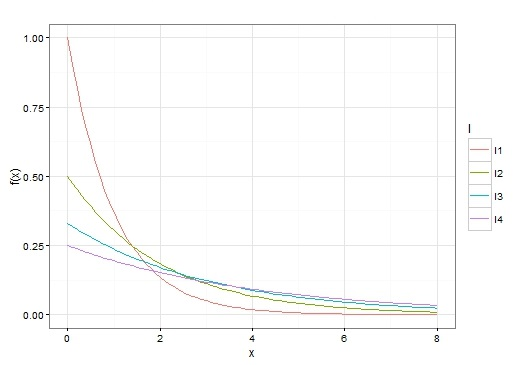
\includegraphics[width=0.85\linewidth]{Figuras/gammadifernetelambda}
	\caption{Distribución gamma con diferente parámetro $\lambda$}
	\label{fig:gammadifernetelambda}
\end{figure}

En la gráfica \ref{fig:gammaalfa} se muestran cuatro distribuciones gamma con al mismo parámetro de escala $\lambda=1$, pero con distintos parámetros de forma, es decir, con $\alpha_{1}=1$, $\alpha_{2}=2$, $\alpha_{3}=3$ y $\alpha_{4}=4$, respectivamente. Adviertase que conforme $\alpha$ es menor el sesgo de la distribución aumenta a la derecha, mientras que si es menor disminuye a la derecha y aumenta a la izquierda. 

\pagebreak

\begin{figure}
	\centering
	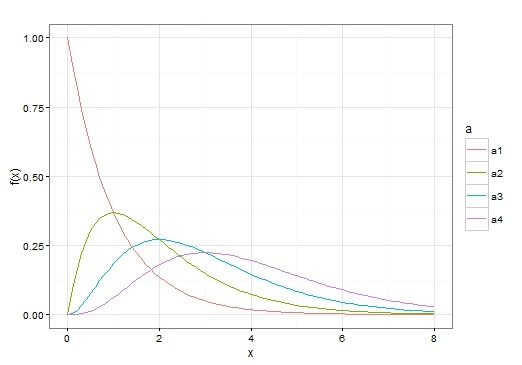
\includegraphics[width=0.8\linewidth]{Figuras/gammaalfa}
	\caption{Distribución gamma con diferente parámetro $\alpha$}
	\label{fig:gammaalfa}
\end{figure}

Si la variable aleatoria $X$ se distribuye gamma con parámetros $\lambda$, $\alpha$, entonces:
%\begin{enumerate}
%	\item \begin{equation*}
%	E[x]=\frac{\alpha}{\lambda}
%	\end{equation*}
%	\item \begin{equation*}
%	Var[x]=\frac{\alpha}{\lambda^{2}}
%	\end{equation*}
%	\item \begin{equation*}
%	m_{x}(t)=(\frac{\lambda}{\lambda-t})^{\alpha}
%	\end{equation*}
%	\item \begin{equation*}
%	\Phi_{x}(it)=(\frac{\lambda}{\lambda-it})^{\alpha}
%	\end{equation*}
%\end{enumerate}
\begin{eqnarray}
	E[x]&=&\frac{\alpha}{\lambda}, \nonumber\\
	Var[x]&=&\frac{\alpha}{\lambda^{2}}, \nonumber\\
	m_{x}(t)&=&(\frac{\lambda}{\lambda-t})^{\alpha},\nonumber\\
	\Phi_{x}(it)&=&(\frac{\lambda}{\lambda-it})^{\alpha}, \nonumber\\
\end{eqnarray}

Por último, es importante mencionar que la distribución gamma es la distribución a priori conjugada de la distribución wishart, la cual se intruduce más adelante.

\section{Distribución gamma inversa}

La distribución gamma inversa resulta de aplicar la transformación $X=\frac{1}{y}$ a la variable aleatoria $Y$, donde $Y$ se distribuye gamma con parámetros $\lambda$ y $\alpha$. Dicho lo anterior se tiene la siguiente definición.

Se dice que una variable aleatoria $X$, que toma valores en los números reales positivos, se distribuye gamma inversa con parámetros $\lambda$ y $\alpha$, si su función de densidad de probabilidad es de la siguiente manera:

\begin{equation}
	f_{x}(x|\lambda, \alpha)=\frac{\lambda^{\alpha}x^{1-\alpha}}{\gamma(\alpha)}\exp\{-\frac{\lambda}{x}\}I_{(0,\infty)}(x).
\end{equation}

La distribución gamma inversa hereda sus dos parámetros de la distribución gamma, por lo que tanto $\lambda$ como $\alpha$ tienen las mismas restricciones que en la distribución gamma, y también caracterizan la forma de la distribución. Al igual que en la distribución gamma, el parámetro $\lambda$ es conocido como parámetro de escala e influye en el tamaño de la densidad respecto al eje $y$. Mientras que el parámetro $\alpha$ influye en la forma de la distribución. 

Para referirnos a que $X$ se distribuye gamma inversa con parámetros $\lambda$ y $\alpha$, usaremos la notación $X|\lambda,\alpha$ se distribuye $\Gamma Inv(x|\lambda,\alpha)$.

Como se mencionó anteriormente, el parámetro $\lambda$ es un parámetro de escala, mientras que el parámetro $\alpha$ es un parámetro de forma, lo cual se ilustra a continuación.

En la gráfica \ref{fig:invgammalambda} se muestran cuatro distribuciones gamma inversa con el mismo parámetro de forma $\alpha=1$, pero con distintos parámetros de escala, es decir, con $\lambda_{1}=1$, $\lambda_{2}=2$, $\lambda_{3}=3$ y $\lambda_{4}=4$, respectivamente. 

\begin{figure}[ht]
	\centering
	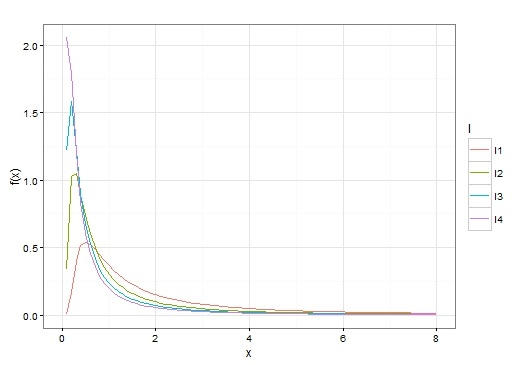
\includegraphics[width=1\linewidth]{Figuras/invgammalambda}
	\caption{Distribución gamma inversa con diferente parámetro $\lambda$}
	\label{fig:invgammalambda}
\end{figure}

En la gráfica \ref{fig:invgammaalfa} se muestran cuatro distribuciones gamma inversa con al mismo parámetro de escala $\lambda=1$, pero con distintos parámetros de forma, es decir, con $\alpha_{1}=1$, $\alpha_{2}=2$, $\alpha_{3}=3$ y $\alpha_{4}=4$, respectivamente. Adviertase que conforme $\alpha$ es menor la curtosis de la distribución aumenta, mientras que si es mayor disminuye.

\newpage
\begin{figure}[ht]
	\centering
	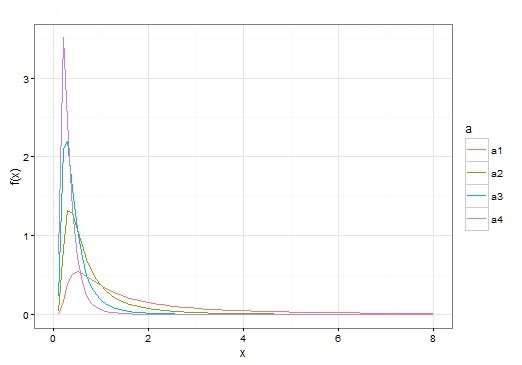
\includegraphics[width=0.9\linewidth]{Figuras/invgammaalfa}
	\caption{Distribución gamma inversa con diferente parámetro $\alpha$}
	\label{fig:invgammaalfa}
\end{figure}


Si la variable aleatoria $X$ se distribuye gamma inversa con parámetros $\lambda$, $\alpha$, entonces:
% \begin{enumerate}
%	\item \begin{equation*}
%	E[x]=\frac{\alpha}{\alpha - 1}
%	\end{equation*}
%	\item \begin{equation*}
%	Var[x]=\frac{\lambda^{2}}{(\alpha-1)^{2}(\alpha-1)}
%	\end{equation*}
%	\item \begin{equation*}
%	\Phi_{x}(it)=(\frac{2(-\lambda it)^{\alpha/2}}{\gamma (\alpha)})\kappa(\sqrt{-4\lambda it})
%	\end{equation*}

%\end{enumerate}
\begin{eqnarray}
	E[x]&=&\frac{\alpha}{\alpha - 1}, \nonumber\\
	Var[x]&=&\frac{\lambda^{2}}{(\alpha-1)^{2}(\alpha-1)},\nonumber\\
	\Phi_{x}(it)&=&(\frac{2(-\lambda it)^{\alpha/2}}{\gamma (\alpha)})\kappa(\sqrt{-4\lambda it}),\nonumber\\
\end{eqnarray}

Por último, es importante mencionar que la distribución Gamma Inversa es la distribución apriori conjugada de la distribución Wishart Inversa, la cual se intruduce más adelante.

\pagebreak
\section{Distribución Wishart}

La distribución whishart es utilizada como distribución de la matriz de varianza-covarianza de
vectores aleatorios normales de dimensión $p$, y se deriva de la siguiente manera:

Supongamos que tenemos $n$ vectores aleatorios $X$  de dimensión $p$ que se distribuyen $N_{p}(X|0,\Sigma)$, luego un estimador de la matriz de varianza-covarianza es $S=\Sigma_{i=1}^{n}x_{i}x_{i}/n$, que es una matriz positiva y simétrica de dimensión $p\times p$, por lo que para los distintos valores que tomen los vectores aleatorios $X$, $S$ también tomará un valor diferente, por lo que es natural preguntarse por la distribución de $S$, con lo cual se llega a la siguiente caracterización. 

Se dice que una matriz $S$ de dimensión $pxp$, simétrica y positiva definida, se distribuye wishart con $n$ grados de libertad, si su densidad es de la siguiente forma:
\begin{equation*}
	f_{S}(S|\Sigma,n,p)= c\frac{|S|^{(n-p-1)/2}}{|\Sigma|^{n/2}}\exp(-\frac{1}{2}tr(\Sigma^{-1}S)),
\end{equation*}

donde $c=\left(2^{np/2}\pi ^{p(p-1)/4}\prod_{i=1}^{p}\gamma(\dfrac{n+1-i}{2})\right)^{-1}$, $\Sigma$ es una matriz simétrica y positiva definida de dimensión $pxp$, y se le conoce como matriz de escala, $n$ es elnúmero de vectores disponibles, y es mayor a la dimensión de los vectores, es decir, mayor que $p$. En este caso usaremos la notación $S$ se distribuye $W(S|\Sigma,n,p)$.\\

Algunas características numéricas de la distribución Whisart son las siguientes:

%\begin{enumerate}
%\item 
\begin{equation*}
	E[S]=p\Sigma,
\end{equation*} \nonumber\\
%\item 
La distribución marginal del $i$-ésimo componente de la distribución wishart se distribuye $\Gamma$($\frac{1}{2}$,$\frac{1}{2}$).\nonumber

%\end{enumerate}




\section{Distribución Wishart inversa}
Se dice que una matriz $G$ de dimensión $p \times p$, simétrica y positiva definida, se distribuye wishart inversa con $n$ grados de libertad, si su función de densidad es de la siguiente forma:
\begin{equation*}
	f_{G}(G)=c\frac{|K|^{(n-p-1)/2}}{|G|^{n/2}}\exp(-\frac{1}{2}tr(G^{-1}K)),
\end{equation*}
donde $c=\left(2^{(n-p-1)p/2}\pi^{p(p-1)/4}\prod_{i=1}^{p}\gamma(\frac{n-p-i}{2})\right)^{-1}$, $K$ es una matriz simétrica y definida positiva, y se le conoce como matriz de escala. En este caso usaremos la notación $G$ se distribuye $W^{-1}(G|K,n,p)$.\\

Una propiedad importante que liga a la distribución wishart y wishart inversa, es la siguiente.\\ 

Si una matriz aleatoria $\Sigma$ de dimensión $p\times p$ se distribuye whisart con matriz de escala $S$, y con $n$ grados de libertad, entonces su matriz inversa, $\Sigma^{-1}$, se distribuye whisart inversa con matriz de escala $S^{-1}$, y con $n+p+1$ grados de libertad.

\section{Distribución gaussiana inversa generalizada}
Se dice que la variable aleatori $X$, que toma valores en los números reales positivos, tiene una distribución gaussiana inversa generalizada, denotada por $GIG(x|\lambda,\xi,\Psi)$, si su densidad es de la siguiente forma:

\begin{equation*}
	f(x)= \dfrac{\xi^{-\lambda}\sqrt{\xi\Psi}^{\lambda}x^{\lambda-1}\exp{\frac{-1}{2}(\xi x^{-1} + \Psi x)}}{2\kappa_{\lambda}(\sqrt{\xi\Psi})}I_{(0,\infty)}(x),  
\end{equation*}
donde $\kappa_{\lambda(.)}$ es una función modificada de Bessel de tercer tipo, y si $\lambda<0$, entonces $\xi>0$, $\Psi \ge 0 $; si $\lambda=0$, entonces $\xi>0$, $\Psi > 0 $, si $\lambda>0$, entonces $\xi\ge 0$, $\Psi > 0 $.\\

En la distribución gaussiana inversa generalizada tres parámetros caracterizan la forma de la distribución. Tanto el parámetro $\xi$ como el parámetro $\Psi$ influyen en la escala de la distribución, mientras que el parámetro $\lambda$ en la forma. El punto anterior se ilustra a continuación.\\

En la gráfica \ref{fig:gigdiferentesvaloresdepsi} se muestran cuatro distribuciones GIG, todas con los mismos parámetros $\lambda=1$ y $\xi=1$, pero con diferentes parámetros $\psi_{1}=0.5$, $\psi_{2}=1$, $\psi_{3}=2$ y $\psi_{4}=4$, respectivamente. Es importante notar que entre menor es el valor de $\psi$, mayor es la curtosis de la distribución. \\


\begin{figure}[ht]
	\centering
	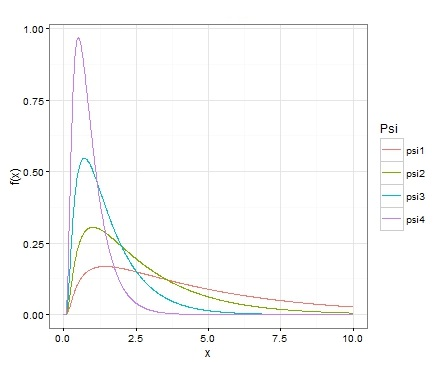
\includegraphics[width=0.8\linewidth]{Figuras/gigdiferentesvaloresdepsi}
	\caption{Distribución GIG con diferentes valores del parámetro $\psi$.}
	\label{fig:gigdiferentesvaloresdepsi}
\end{figure}

En la gráfica \ref{fig:gigcondiferentesvaloresdexi} se observan cuatro distribuciones GIG, todas con paámetros $\lambda=1$ , $\psi=1$, pero con diferentes parámetros $\xi_{1}=0.5$, $\xi_{2}=1$, $\xi_{3}=2$ y $\xi_{4}=4$, respectivamente. Es importante notar que entre mayor es el valor del parámetro $\xi$, mayor es el sesgo a la derecha de la distribución.

\newpage
\begin{figure}[ht]
	\centering
	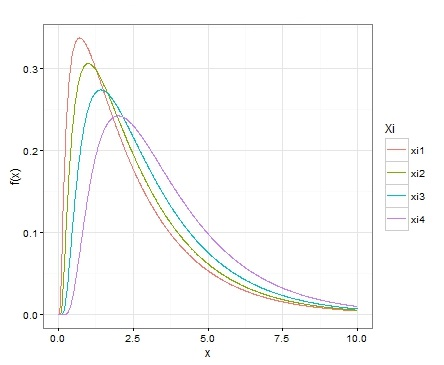
\includegraphics[width=0.8\linewidth]{Figuras/gigcondiferentesvaloresdexi}
	\caption{Distribución GIG con diferentes valores del parámetro $\xi$}
	\label{fig:gigcondiferentesvaloresdexi}
\end{figure}

En la gráfica \ref{fig:gigdiferentesvaloreslambda} se observan cuatro distribuciones GIG, todas con parámetros $\psi=1$ , $\xi=1$, pero con diferentes parámetros $\lambda_{1}=-0.5$, $\lambda_{2}=0$, $\lambda_{3}=.5$ y $\lambda_{4}=1$, respectivamente. En este caso el parámetro $\lambda$ también influye en la curtosis de la distribución, ero sobre todo influye en la cola de esta. También el parámetro $\lambda$ influye en la failia paramétrica, pues si la variable aleatoria $X$ se distribuye GIG, con parámetro $\lambda=0$ entonces se obtiene la distribución hiperbólica, mientras que si $\lambda=-0.5$ se obtiene la distribución Gaussiana Inversa de la cual se hablará posteriormente. 

\newpage 
\begin{figure}[ht]
	\centering
	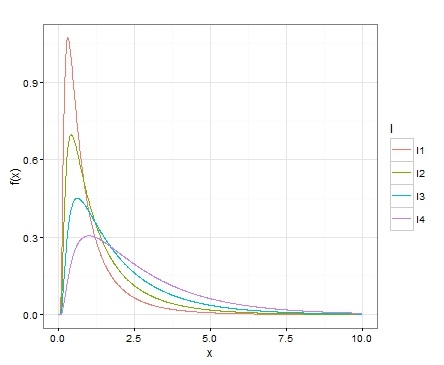
\includegraphics[width=0.8\linewidth]{Figuras/gigdiferentesvaloreslambda}
	\caption{Distribución GIG con diferentes valores de $\lambda$}
	\label{fig:gigdiferentesvaloreslambda}
\end{figure}


Ahora veamos algunos resultados de la distribución GIG. Si $X$ se distribuye $N\tilde{}(x|\lambda,\xi,\Phi)$, entonces su función generadora de momentos es:

\begin{eqnarray*}
\Phi (it) & = &\underset{-\infty }{\overset{\infty }{\int }}\exp(itx){\dfrac{\xi^{-\lambda}\sqrt{\xi\Psi}^{\lambda}x^{\lambda-1}\exp{\frac{-1}{2}(\xi x^{-1} + \Psi x)}}{2\kappa_{\lambda}(\sqrt{\xi\Psi})}}dx\\
 &=& c\underset{-\infty }{\overset{\infty }{\int }}\xi^{-\lambda}\frac{\sqrt{\xi(2it + \Psi)}^{\lambda}}{2\kappa_{\lambda}(\sqrt{\xi(2it + \Psi)})}\exp{\frac{-1}{2}(\xi x^{-1} + (2it+\Psi) x)}dx,\\ 
\end{eqnarray*}

con $c=\frac{\sqrt{\xi\Psi}^{\lambda}}{2\kappa_{\lambda}(\sqrt{\xi\Psi})}\frac{2\kappa_{\lambda}(\sqrt{\xi(2it + \Psi)})}{\sqrt{\xi(2it + \Psi)}^{\lambda}}$. La última integral vale uno por ser una densidad $N\bar{}(\lambda,\xi,2it + \psi)$ integrada sobre su soporte, por lo que:

\begin{equation*}
	\Phi(it)=\frac{\sqrt{\xi\Psi}^{\lambda}}{\kappa_{\lambda}(\sqrt{\xi\Psi})}\frac{\kappa_{\lambda}(\sqrt{\xi(2it + \Psi)})}{\sqrt{\xi(2it + \Psi)}^{\lambda}}.
\end{equation*}

Si $X$ se distribuye $N\tilde{}(x|\lambda,\xi,\Phi)$, entonces su $r$-ésimo momento es:
\begin{equation*}
	E[X^{r}]=\underset{-\infty }{\overset{\infty }{\int }}x^{r}\dfrac{\xi^{-\lambda}\sqrt{\xi\Psi}^{\lambda}x^{\lambda-1}\exp{\frac{-1}{2}(\xi x^{-1} + \Psi x)}}{2\kappa_{\lambda}(\sqrt{\xi\Psi})}dx
\end{equation*}
\begin{equation*}
	=\frac{x^{r}2\kappa_{\lambda+r}(\sqrt{\xi\Psi})}{\sqrt{\xi\Psi}^{r}2\kappa_{\lambda}(\sqrt{\xi\Psi})}\underset{-\infty }{\overset{\infty }{\int }}\dfrac{\xi^{-\lambda-r}\sqrt{\xi\Psi}^{\lambda+r}x^{\lambda+r-1}\exp^{{\frac{-1}{2}(\xi x^{-1} + \Psi x)}}}{2\kappa_{\lambda+r}(\sqrt{\xi\Psi})}dx
\end{equation*}
Por lo tanto:
\begin{equation*}
	E[X^{r}]=(\frac{\xi}{\Psi})^{\frac{r}{2}}\frac{\kappa_{\lambda+r}(\sqrt{\xi \Psi})}{\sqrt{\kappa_{\lambda}(\sqrt{\xi\Psi})}}
\end{equation*}

\section{Distribución gaussiana inversa}
Se dice que la variable aleatoria $X$ tiene una distribución gaussiana inversa si su función de densidad es de la siguiente forma:
\begin{equation*}
	f_{x}(X|\lambda,\psi)=\sqrt{\dfrac{\lambda}{2\pi x^{3}}}\exp(-\dfrac{\lambda(x-\Psi)^{2}}{2\Psi^{2}x}),
\end{equation*}
para $\lambda$, $\psi$ y $X$ mayores a cero.
Como notación, si X se distribuye gausiana inversa con parámetros $\lambda$, $\Psi$, diremos que $X|\lambda,\psi$ se distribuye $GI(X|\lambda,\Psi)$.

Ahora veamos como es la función característica de esta distribución.
Si $X$ se distribuye $GI(x|\lambda,\Psi)$, entonces su función característica es:

\begin{equation}
	\begin{split} \label{211}
		\Phi_{x}(it)& =\int_{0}^{\infty}\exp^{itx}\sqrt{\dfrac{\lambda}{2\pi x^{3}}}\exp^{-\dfrac{\lambda(x-\Psi)^{2}}{2\Psi^{2}x}}dx\\
		&=\int_{0}^{\infty}\sqrt{\dfrac{\lambda}{2\pi x^{3}}}\exp(-\dfrac{\lambda}{2\Psi^{2}}(x-2\Psi-(itx2\Psi^{2}/\lambda)+\Psi^{2}x))dx\\
	\end{split}
\end{equation}
Trabajando únicamente con el exponente de la expresión anterior, y factorizando el término
$(1-\frac{it2\Psi^{2}}{\lambda})$ tenemo que:
\begin{equation} \label{212}
	\begin{split}
		%-\dfrac{\lambda}{2\Psi^{2}}(x-2\Psi-(itx2\Psi^{2}/\lambda)+\Psi^{2}x)  =
		&-\frac{\lambda}{2\Psi^{2}}(1-\frac{it2\Psi^{2}}{\lambda})
		(x-2\Psi/(1-\frac{it2\Psi^{2}}{\lambda})
		+\Psi^{2}/(1-\frac{it2\Psi^{2}}\lambda)\\ 
		&=-\dfrac{\lambda}{2\Psi^{2}}(1-\frac{it2\Psi^{2}}{\lambda})(x-2\Psi/(1-\frac{it2\Psi^{2}}{\lambda})
		+\Psi^{2}/x(1-\frac{it2\Psi^{2}}{\lambda})\\
		&+2\Psi/\sqrt{1-\frac{it2\Psi^{2}}{\lambda}}
		-2\Psi/\sqrt{1-\frac{it2\Psi^{2}}{\lambda}})\\
		&=\frac{\lambda}{\Psi}-\frac{\lambda}{\Psi}\sqrt{(1-\frac{it2\Psi^{2}}{\lambda})}-
		\frac{\lambda}{2x\Psi^{2}}(1-\frac{it2\Psi^{2}}{\lambda})(x
		-\Psi/\sqrt{1-2it\Psi^{2}/\lambda})^{2}
	\end{split}
\end{equation}

Por lo que la función característica queda de la siguiente forma:
\begin{eqnarray*}
\Phi_{x}(it) & =& (\exp^{\frac{\lambda}{\Psi}-\frac{\lambda}{\Psi}\sqrt{(1-\frac{it2\Psi^{2}}{\lambda})}}) \\
& &(\int_{0}^{\infty}\sqrt{\dfrac{\lambda}{2\pi x^{3}}}\exp^{\frac{\lambda}{2x\Psi^{2}}(1-\frac{it2\Psi^{2}}{\lambda})(x
	-\Psi/\sqrt{1-2it\Psi^{2}/\lambda})^{2}}dx)\\
&=&\exp(\frac{\lambda}{\Psi}-\frac{\lambda}{\Psi}\sqrt{(1-\frac{it2\Psi^{2}}{\lambda})})\\
\end{eqnarray*}


%\begin{equation}
%	\begin{split} \label{213}
%		\Phi_{x}(it)& =\exp^{\frac{\lambda}{\Psi}-\frac{\lambda}{\Psi}\sqrt{(1-\frac{it2\Psi^{2}}{\lambda})}} \int_{0}^{\infty}\sqrt{\dfrac{\lambda}{2\pi x^{3}}}\exp^{\frac{\lambda}{2x\Psi^{2}}(1-\frac{it2\Psi^{2}}{\lambda})(x
			%-\Psi/\sqrt{1-2it\Psi^{2}/\lambda})^{2}}dx\\
		%&=\exp^{\frac{\lambda}{\Psi}-\frac{\lambda}{\Psi}\sqrt{(1-\frac{it2\Psi^{2}}{\lambda})}}
	%\end{split}
%\end{equation}

El resultado anterior se sigue de que la integral previa es una distribución Gaussiana Inversa con parámetros $\lambda$, $\Psi/\sqrt{1-(2it\Psi^{2})/\lambda}$ integrada sobre su soporte, por lo cual vale $1$, y por lo tanto:
\begin{equation}
	\Phi_{x}(it)=\exp^{\frac{\lambda}{\Psi}-\frac{\lambda}{\Psi}\sqrt{(1-\frac{2it\Psi^{2}}{\lambda})}}
\end{equation}

Con el resultado anterior se puede probar que si $X$ se distribuye $GI(x|\lambda,\Psi)$, entonces:
%\begin{enumerate}
%	\item \begin{equation*}
%m_{x}(t)=\exp^{\frac{\lambda}{\Psi}-\frac{\lambda}{\Psi}\sqrt{(1-\frac{2t\Psi^{2}}{\lambda})}}
%\end{equation*}
%\item \begin{equation*}
%E[X]=\Psi
%\end{equation*}
%\item \begin{equation*}
%Var[X]=\frac{\Psi^{3}}{3}
%\end{equation*}
%\item \begin{equation*}
%Sesgo[X]=\frac{2\Psi^{4}}{\lambda}+\frac{3\Psi^{5}}{\lambda^{2}}
%\end{equation*}
%\end{enumerate}
\begin{eqnarray}
	m_{x}(t)= \exp^{\frac{\lambda}{\Psi}-\frac{\lambda}{\Psi}\sqrt{(1-\frac{2t\Psi^{2}}{\lambda})}},
	&&
	E[X]=\Psi,
	\nonumber\\
	Var[X]=\frac{\Psi^{3}}{3},
	&&
	Sesgo[X]=\frac{2\Psi^{4}}{\lambda}+\frac{3\Psi^{5}}{\lambda^{2}}.
	\nonumber
\end{eqnarray}

Entoces, al igual que la distibución gaussiana, la distribución gaussiana inversa tiene un parámetro de localización, es decir, $\Psi$. Es importante notar como afecta el parámetro $\lambda$ a la dispersión de la variable aleatpria $X$, y además, esta distribución siempre tiene un sesgo positivo ya que $\Psi$ y $\lambda$ son mayores a cero. Por lo que para valores muy pequeños de $\lambda$ o muy grandes de $\Psi$ la distribución tendrá más peso en la cola. 

%\citep{Abadie_DifferencesinDifferences}

%\citeauthor{AbadieGardeazabal_EconCostConflict}

%\citeyear{Abadie_etal_SyntheticControlComparative}

%\begin{figure}[htbp]
%	\centering
%	\caption{Una gr\'afica....}
%	\label{fig_ejemplo}
%		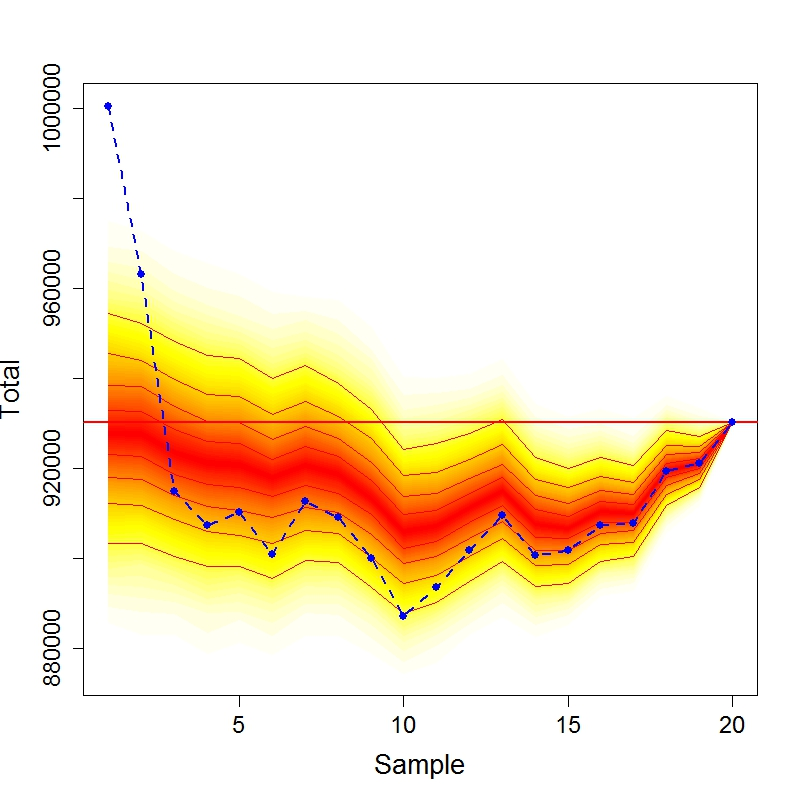
\includegraphics[width=0.97\textwidth]{Figuras/Ejemplo_Figura.jpg}
%\end{figure}

%
%	Table 1.
%
%\begin{table}[H]
%\begin{center}
%\begin{threeparttable}
%	\caption{Una tabla}
%	\label{tab_ejemplo}
%	{\scriptsize
%	\begin{tabular}{l c c c c c c c c c}
%		\toprule
%		\hline
%										& \multicolumn{9}{c}{Year}  \\
%		State		 			& 2003	& 2004	& 2005	& 2006	& 2007	& 2008	& 2009	& 2010	& 2011 \\
%		\midrule
%		\hline
%		\hline
%		Uno 		& 1.1	& 1.0	& 1.0	& 1.1	& 1.1	& 1.0	& 1.1	& 1.1	& 1.1 \\
%		Dos 		& 3.0	& 3.0	& 3.0	& 3.0	& 2.9	& 2.8	& 2.8	& 2.7	& 2.7 \\
%		\bottomrule
%		\hline
%	\end{tabular}
%	\begin{tablenotes}
%		\tiny
%		\item Source: ...
%		\item Note: ...
%	\end{tablenotes}
%	}			
%\end{threeparttable}
%\end{center}
%\end{table}
%\chapter{Mezclas de distribuciones gausianas}

En este cap\'itulo primero se hablar\'a en t\'erminos generales sobre qu\'e es una distribuci\'on tipo mezcla. Despu\'es se hablar\'a de un caso particular de las distribuciones tipo mezcla continua, es decir, de las distribuciones tipo mezcla normal (McNeil et al, 2015). Para despu\'es caracterizar a la distribuci\'on hiperb\'olica generalizada a partir de una distribuci\'on tipo mezcla. Por \'ultimo, se aprovechar\'an algunas propiedades de las distribuciones tipo mezcla normal, para obtener algunas caracter\'isticas de inter\'es de la distribuci\'on hiperb\'olica generalizada.

\section{Distribuciones tipo mezcla }
Este tipo de distribución consiste en ponderarar un conjunto numerable de vectores aleatorios $X_{i}$  discretos con el mismo soporte y la misma dimensión con un conjunto de pesos $w_{i}$, positivos y menores a uno, $w_{i}$, donde $i$ proviene de un conjunto $I$ de índices numerable, y a su vez $\sum_{i\in I}w_{i}=1$. El índice $i$ puede ser generado por una distribución de probabilidad discreta tal que $P(i)=w_{i}$; por ello a los pesos también se les conoce como probabilidades. Entonces la función de densidad es de la siguiente forma:\\

\begin{equation*}
f_{x}(x)= \sum_{i\in I}w_{i}f_{X_{i}}(x)
\end{equation*}
Donde  $0<w_{i}<1$, $\sum_{i\in I}w_{i}=1,$ y $  f_{X_{i}}(x)$ es un vector aleatorio discreto de dimensión p para todo $i$ en $I$.\\

Es común encontrar este tipo de distribuciones en un conjunto de datos que provienen de dos o más distribuciones diferentes, lo cual podría resultar en una distribución multimodal. Si el conjunto de vectores aleatorios provienen de la misma distribución, entonces se dice que es una mezcla de familias paramétricas, mientras que si el vector aleatorio tiene una distribución continua se le conoce como densidad tipo mezcla continua.\\
Una densidad tipo mezcla continua resulta de considerar que los pesos $w$ están dados por una densidad continua $f_{w}(w)$ con soporte en $R_{+}$; a $w$ se le conoce como variable de mezcla. Ahora, el vector aleatorio $X$ está parametrizado por $(\theta,w)$, por lo que la familia de vectores aleatorios queda determinada por la familia no numerable  $ X$ dado $w$, con $w$ distribuido $f_{w}(w) $. Entonces, la densidad de $X$ esté dada por:\\
\begin{equation*}
f_{x}(x)=\int_{0}^{\infty}f(x|w)f_{w}(w)dw 
\end{equation*}


Si $w$ es una variable aleatoria con distribución paramétrica, es común que la distribución de $X$ dependa de los parámetros de $u$, y además ciertas características como la dispersión o la cola de la distribución de $X$ también dependan de las características de la variable de mezcla $w$.\\

\section{Mezcla gaussiana en media}
Se dice que un vector aleatorio $X$, de dimensión $p$, es una mezcla en media si, dado $u$, $X$ tiene una distribución gaussiana con vector de  medias $u\mu$, y matriz de varianza-covarianza $\Sigma$. La variable aleatoria $u$ está definida en $R_{+}$. Entonces la probabilidad de que $X$ pertenezca a algún subconjunto $S_{p}\subset  R^{p}$ es:

\begin{equation*}
P((X_{1},...,X_{p})\in S_{p})=\underset{0}{\overset{\infty }{\int }}N_{p}(X \in S_{p} |u\mu,\Sigma)f_{u}(u)du, 
\end{equation*}
donde  $\mu \in R^{p}$, $\Sigma \in M_{p\times p}$ y $u$ es la variable de mezcla.\\
Si nos enfocamos en la distribución marginal de $X$ dado $u$ podemos notar que el valor de $u$ influye en donde está centrada la distribución, pues ahora el vector de medias pertenece al segmento dirigido $L(\mu)=( u\mu | u\in R_{+}, \mu\in R^{p})$. Entonces, si consideramos que $u$ ha tomado el valor de $u_{i}$, y una muestra aleatoria de $X$ dado $u_{i}$, tendremos una muestra centrada sobre el segmento dirigido $L(\mu)$ en el punto $u_{i}\mu$, por lo que para valores de $u$ cercanos a uno, la muestra permanece centrada al rededor de $\mu$, mientras que para valores grandes de $u$, la muestra se aleja en dirección del vector de medias $\mu$. \\


En la gráfica (\ref{fig:RplotG}) se ilustra la simulación de una distribución tipo mezcla gaussiana con vector de medias $\mu=(9,11)$, matriz de varianza-covarianza $\Sigma$, con entradas $\sigma_{1}=\sigma_{2}=5$, y $\sigma_{1,2}=\sigma_{2,1}=0.1$
%$\left(
%\begin{array}{lcr}
%5 & .1 \\ .1 & 5
%\end{array}\right) $
, y con variable de mezcla distribuida exponencialmente, para tres diferentes valores de $u$. Obsérvese que para cada valor que tomó la variable de mezcla $u$, las realizaciones del vector aleatorio $X$ dado $u$ se concentrán al rededor 
de algún punto del vector de medias $u\mu$.\\   

\begin{figure}[h]
	\centering
	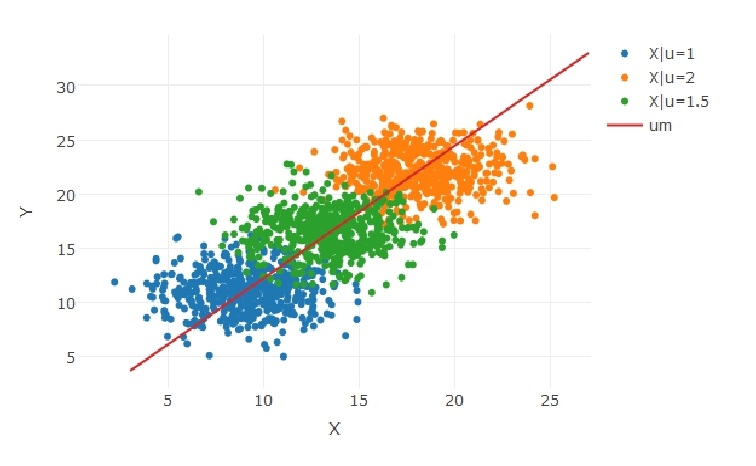
\includegraphics[width=1.15\linewidth]{Figuras/RplotG}
	\caption{Mezcla en media}
	\label{fig:RplotG}
\end{figure}

%En la gráfica (\ref{fig:mm}) se observa como tanto la función de densidad, como los contornos del vector aleatorio $X$ dado $u$, se ven afectados por la variable de mezcla $u$, para tres diferentes valores de $u$.\\

\begin{figure}[h]
	\centering
	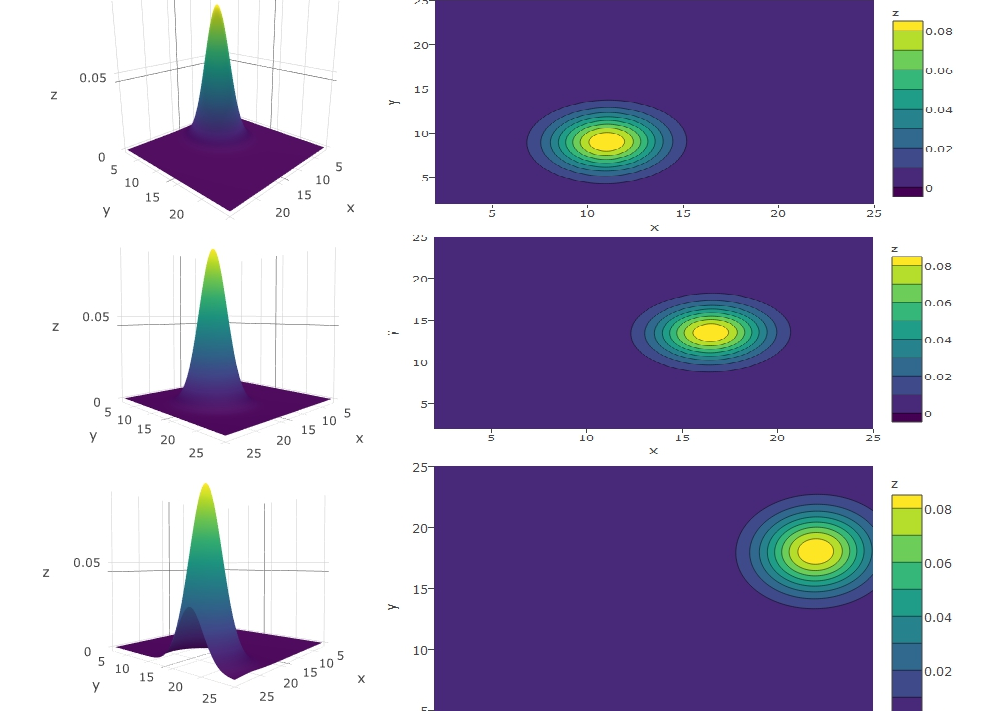
\includegraphics[width=1.15\linewidth]{Figuras/mm}
	\caption{Contornos de una distribución tipo mezcla normal en media.}
	\label{fig:mm}
\end{figure}

\pagebreak
En la gráfica (\ref{fig:mm}) se observa como tanto la función de densidad, como los contornos del vector aleatorio $X$ dado $u$, se ven afectados por la variable de mezcla $u$, para tres diferentes valores de $u$.\\

Ahora veamos analíticamente cómo influyen algunas de las caractarísticas numéricas de la variable de mezcla $u$ en la dispersión del vector aleatorio $X$, por lo que:
%%PONER ESTO EN UN ARRAY
\begin{eqnarray}
E[X]& =&\int_{0}^{\infty} \left( \int_{D_{X}}XN_{p}(X|u\mu,\Sigma)f_{u}(u)du\right)  dx \nonumber\\
&=&\int_{0}^{\infty}f_{u}(u)\left(\int_{D_{X}}XN_{p}(X|u\mu,\Sigma)f_{u}(u)dx\right)du\nonumber\\
&=&\int_{0}^{\infty}f_{u}(u)E[X|u]du\nonumber\\
&=&\int_{0}^{\infty}f_{u}(u)u\mu du\nonumber\\
&=&\mu\int_{0}^{\infty}uf_{u}(u)du\nonumber\\
&=&\mu E[u]\nonumber\\
\end{eqnarray}

%\begin{equation*}
%E[X]=\int_{0}^{\infty} \left( \int_{D_{X}}XN_{p}(X|u\mu,\Sigma)f_{u}(u)du\right)  dx
%\end{equation*}
%\begin{equation*}
%\int_{0}^{\infty}f_{u}(u)\left(\int_{D_{X}}XN_{p}(X|u\mu,\Sigma)f_{u}(u)dx\right)du=\int_{0}^{\infty}f_{u}(u)E[X|u]du
%\end{equation*}
%\begin{equation*}
%\int_{0}^{\infty}f_{u}(u)u\mu du=\mu\int_{0}^{\infty}uf_{u}(u)du=\mu E[u]
%\end{equation*}


Mientras que por el anexo $4$ se tiene que: 
\begin{eqnarray}
Cov(X)&=&E[Cov(X|u)]+Cov[E[X|u]]
\nonumber\\
&=&E[\Sigma]+Cov[u\mu]\nonumber\\
&=&\Sigma + var(u)\mu \mu',\nonumber\\
\end{eqnarray}
siempre y cuando el segundo momento de $X$ y $u$ existan. \\

Así, la variable de mezcla $u$ influye en la localización y dispersión del vector aleatorio $X$; intuitivamente podemos considerar al producto de $u$ con el vector de medias $\mu$ como un sesgo adicional que influye en la realización del vector aleatorio $X$. Este tipo de mezcla nos permite modelar conjuntos de datos que sigan alguna tendencia con disperción constante, como se ilustra en la gráfica (\ref{fig:RplotG}). Por otra parte , una de las mayores dificultades es que, salvo en algunas excepciones, no siempre existe una forma cerrada para la densidad del vector aleatorio $X$, por lo que tendría que ser aproximada mediante algún método númerico.\\

Mediante un proceso de simulación se generaron realizaciones del vector aleatorio $X$ a través de distribuciones tipo mezcla normal, lo cual se ilustra en la gráfica (\ref{fig:abcd}). La gráfica a) proviene de una variable de mezcla Exponencial con parámetro $\lambda=1.5$, la b) proviene de una variable de mezcla Gamma con parámetros $\alpha=20$, $\beta=5$, la c) provine de una variable de mezcla Pareto con parámetros $\theta=5$, $\alpha=2$, y la d) proviene de una variable de mezcla Ji-cuadrada con 20 grados de libertad (el vector aleatorio $X$ dado $u$ se distribuye de la misma manera que en la gráfica (\ref{fig:RplotG})).

\begin{figure}[h]
	\centering
	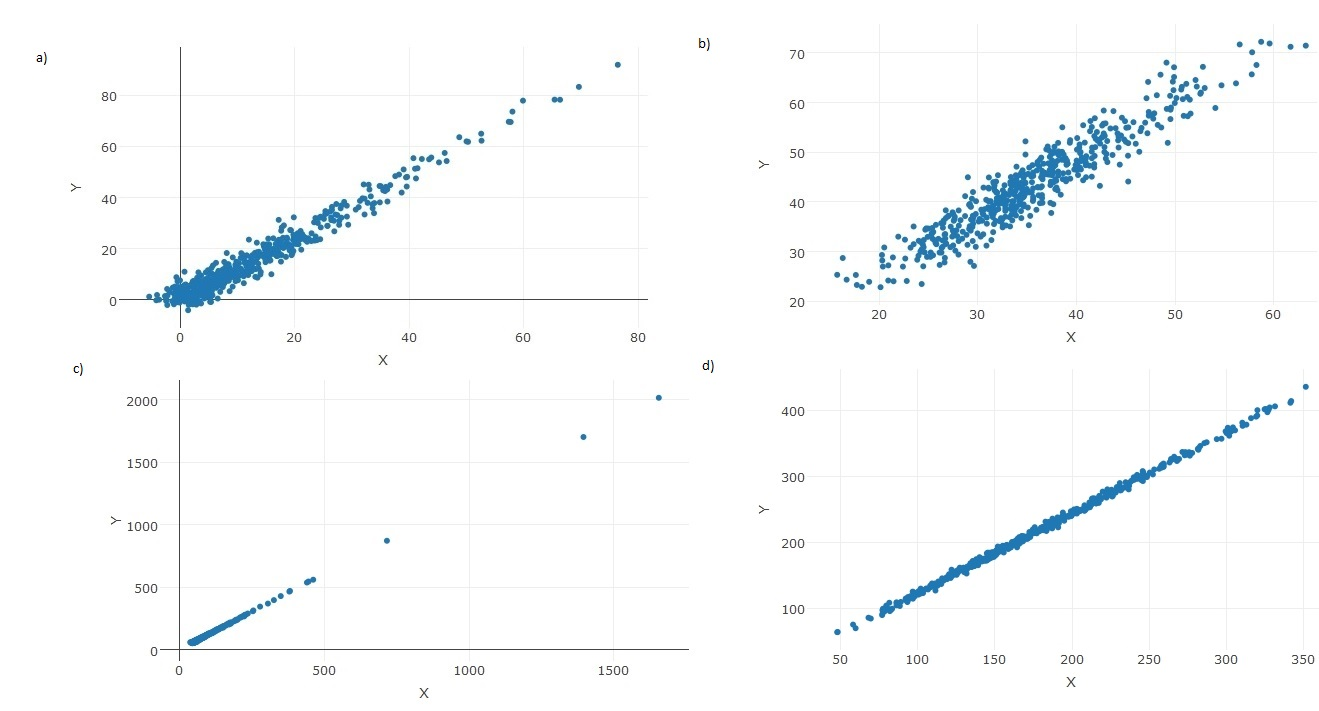
\includegraphics[width=1\linewidth]{Figuras/expo}
	\caption{Simulación del vector aleatorio X a través de distribuciones tipo mezcla normal con diferente variable de mezcla.}
	\label{fig:abcd}
\end{figure}
Como se describió en la gráfica (\ref{fig:RplotG}), las simulaciones del vector aleatorio $X$ parecen seguir una tendencia, y además es importante notar que la dispersión alrededor del vector de tendencia de la gráfica (b) es mayor a la de la gráfica (b). También es importante notar que en la gráfica (c) hay valores aparentemente grandes, mientras que en la gráfica (d) casi todos los valores parecen concentrarse en algún intervalo de la posible recta de tendencia.
Por lo que, intuitivamente la cola de la distribución de $u$ influye en la distribución de $X$. La gráfica (d) proviene de considerar una variable de mezcla distribuida Pareto, la cual tiene cola pesada, y como consecuencia podemos observar gran dispersión sobre el vector de tendencia. Mientras que la gráfica (d) proviene de considerar una variable de mezcla $u$ distribuida Xi cuadrado, que es de cola ligera, y como consecuencia las simulaciones del vector $X$ no están tan dispersas sobre el vector de tendencia (lo mismo podemos decir de la gráfica (a) y (b)).


\section{Mezcla gaussiana en varianza}
Ahora consideremos un modelo similar al anterior, pero con la diferencia que la variable de mezcla u solamente afecta a la matriz de varianza-covarianza $\Sigma$. Luego, la distribución del vector aleatorio $X$ de dimensión $p$ viene dado por:
\begin{equation}
P\left( (X_{1},...,X_{p})\in S_{p} \right )=\underset{0}{\overset{\infty }{\int }}N_{p}(X\in S_{p}|\mu,u\Sigma)f_{u}(u)du 
\end{equation}
En la distribución condicional de $X$ dado $u$, podemos notar que $u$ influye en la disperción de $X$, por lo que entre mayor sea el valor que tome $u$, mayor será la disperción al rededor del vector de medias $\mu$. Como ejemlo, en la gráfica (\ref{fig:mez}) se presenta la simulación de una variable tipo mezcla normal en varianza, con vector de medias $\mu=(9,11)$, matriz de varianza-covarianza $\sigma_{1}=\sigma_{2}=5$, y $\sigma_{1,2}=\sigma_{2,1}=0.1$
%$\Sigma = $
%$\left(
%\begin{array}{lcr}
%5 & .1 \\ .1 & 5
%\end{array}\right) 
%$
, y variable de mezcla $u$ distribuida Exponencial, con parámetro $\lambda=1$.\\      


\begin{figure}[h!]
	\centering
	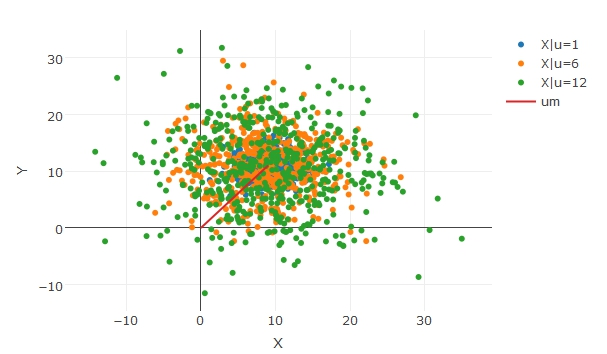
\includegraphics[width=1\linewidth]{Figuras/gvcarregida}
	\caption{Modelo de mezcla normal en varianza.}
	\label{fig:mez}
\end{figure}

\pagebreak
En la gráfica (\ref{fig:contornosv}) se observa cómo se modifican tanto la densidad como los contornos de la densidad de $X$ dado $u$ del ejemplo anterior. Claramente se observa que entre mayor sea el valor de $u$, mayor dispersión tendrá el vector $X$ dado $u$.



\begin{figure}[h]
	\centering
	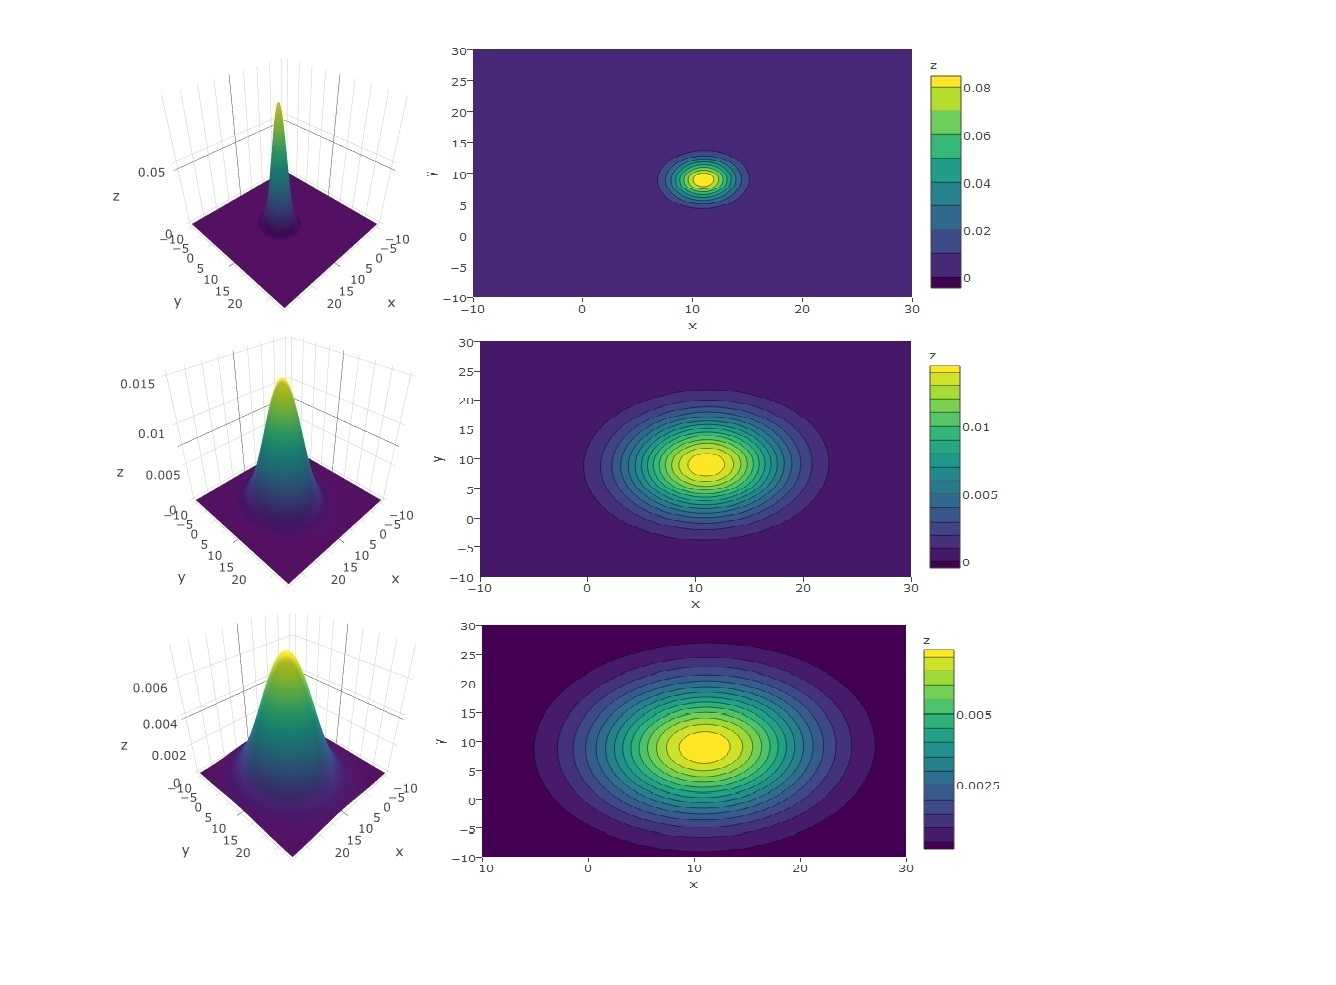
\includegraphics[width=1.15\linewidth]{Figuras/sv1}
	\caption{Contornos de una distribución tipo mezcla normal en varianza}
	\label{fig:contornosv}
\end{figure}
\pagebreak

Ahora considerando algunas características numéricas de $X$, y usando el anexo 4, es fácil probar que si $X$ se puede expresar como una distribución tipo mezcla normal en varianza, entonces: 

%\begin{equation*}
%E[X]=\mu
%\end{equation*}
%\begin{equation*}
%COV[X]=COV_{u}(E_{x}(X|u)) + E_{x}(COV_{u}(X|u))=E(u)\Sigma E(u)'
%\end{equation*}
\begin{eqnarray}
E[X]&=&\mu \nonumber \\
COV[X]&=&COV_{u}(E_{x}(X|u)) + E_{x}(COV_{u}(X|u)) \nonumber\\
&=&E(u)\Sigma E(u)'\nonumber\\
\end{eqnarray} 

Por lo que podemos conocer la esperanza y matriz de varianza-covarianza del vector $X$ con tan sólo conocer la matriz de varianza-covarianza de la distribución de $X$ dado $u$. Además, la distribución del vector $X$ estará centrada en el mismo vector de medias que $X$ dado $u$ para cualquier valor de $u$, mientras que la matriz de varianza-covarianza será proporcional a la matriz de varianza-covarianza de $X$ dado u.\\

En la gráfica (\ref{fig:dmv}) se presentan simulaciones de realizaciones del vector aleatorio $X$ a través de distribuciones tipo mezcla normal en varianza, para ello se utilizaron las mismas distribuciones de mezcla que en la gráfica (\ref{fig:abcd}). Adviértase que, a diferencia del condicionamiento en media, los datos solo se concentran alrededor del vector de medias $\mu$, pues $E[X]=E[X|u]$, perdiendo así la trayectoria que induce el vector de medias; intuitivamente podemos pensar que $u\mu$ del modelo de mezcla en media genera un vector de trayectoria para las observaciones de $X$, y que además induce un sesgo de las observaciones del vector $X$ sobre el vector de tendencia $\mu$.\\

\begin{figure}[h]
	\centering
	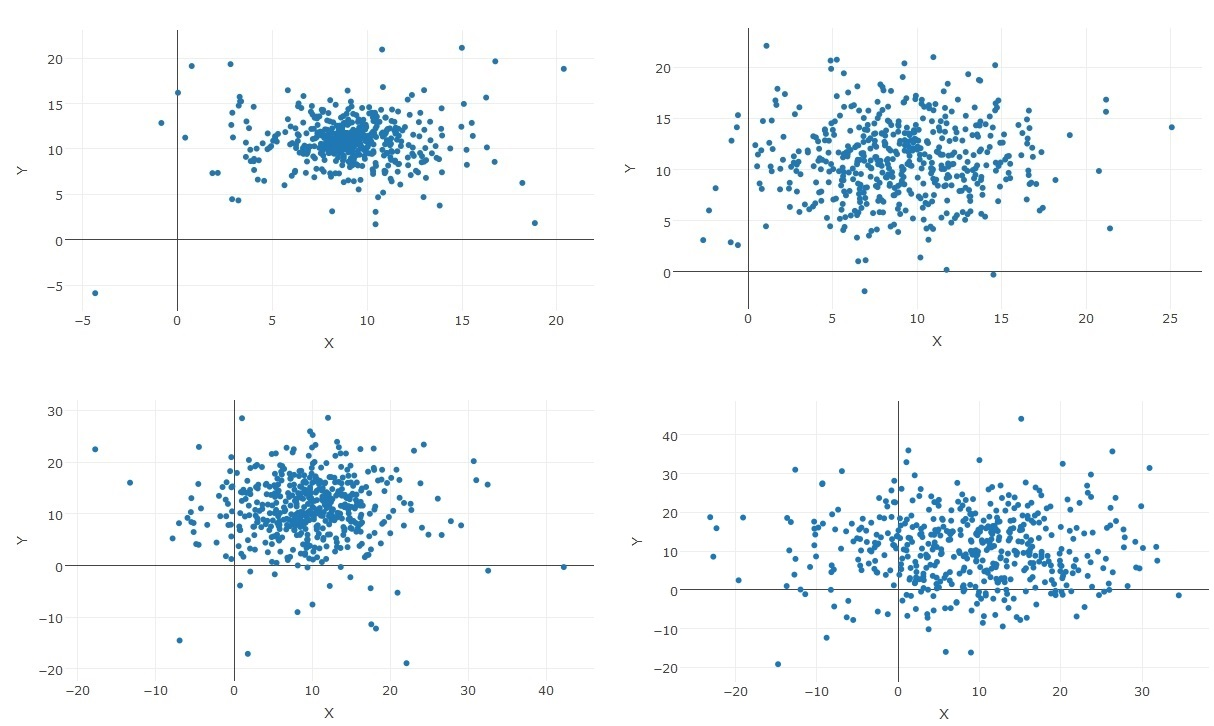
\includegraphics[width=1\linewidth]{Figuras/varianzaexp}
	\caption{Ejemplos de distribuciones tipo mezcla en varianza con diferentes distribuciones de mezcla.}
	\label{fig:dmv}
\end{figure}


\pagebreak
\section{Mezcla gaussiana en media-varianza}

Generalizando los dos modelos anteriores se tiene la siguiente definición:\\

Se dice que un vector aleatorio $X\in R^{p}$ es un vector tipo mezcla p-dimensional, si $X$ dado $u$ se ditribuye Normal con vector de medias $\mu +u\beta$, y matriz de varianza-covarianza $u\Sigma$, donde u es la variable de mezcla con soporte en $R_{+}$, $\mu, \beta \in R^{p}$ y $\Sigma\in M_{p \times p}$ matriz de varianza-covarianza.

Así pues, la distribución del vector $X$ está dada por:

\begin{equation*}
f_{X}(x)=\underset{S_{u}}{\int}\dfrac{1}{(2\pi)^{n/2}|u\Sigma|^{n/2}}\exp(-\dfrac{1}{2}(x-\mu-uB)\acute{}u\Sigma^{-1}(x-\mu-uB))f(u)du 
\end{equation*}

Si nos concentramos en la distribución marginal de $X$ dado $u$, notamos que ahora, para cada realización  $u_{i}$, la densidad de $X$ dado $u_{i}$ estará centrada en el vector $\mu + u_{i}\beta$, y conforme $u_{i}$ tome valores más grandes, la densidad de $X/u_{i}$ se desplazará en dirección del vector $u_{i}\beta$ cada vez con mayor dispersión. 
En la gráfica (\ref{fig:dmnev}) se puede observar una variable tipo mezcla en esperanza varianza, con parámetros $\beta=(9,11)$, $\mu=(5,10)$, y matriz de varianza-covarianza $\Sigma$
con $\sigma_{z}=\sigma_{y}=5$, y $COV(Z,Y)=0$.$1$, donde $X=(Z,Y)$ es un vector aleatorio de dimensión $2$.
%$\left(
%\begin{array}{lcr}
%5 & .1 \\ . 1 & 5
%\end{array}\right) 
. La variable de mezcla $u$ se distribuye exponencial y tomó los valores de $1$, $3$ y $6$ respectivamente.

\begin{figure}[h]
	\centering
	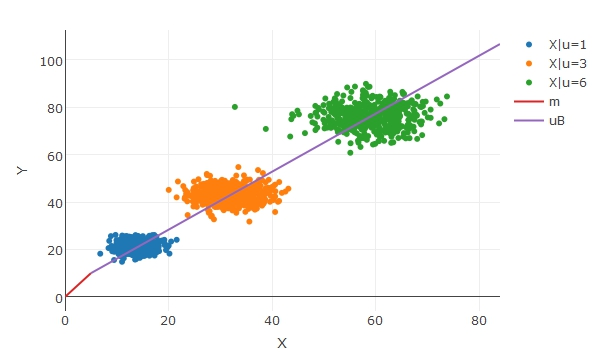
\includegraphics[width=1\linewidth]{Figuras/bm}
	\caption{Gráfica de una variable tipo mezcla normal en esperanza varianza}
	\label{fig:dmnev}
\end{figure}


\pagebreak
En la distribución de $X$ podemos considerar a $\mu$ como un vector de posición, mientras que $u\beta$ es un vector de dirección o tendencia alrededor del cual estarán las observaciones de $X$. Los datos conservarán la estructura de correlación inherenta a $\Sigma$, pero además estarán dispersos en proporción a la esperanza de la variable de mezcla $u$, más alguna constante que depende de $u$. Siguiendo la idea intuitiva del modelo de mezcla en media, el producto de la variable de mezcla $u$ y el vector $\beta$ inducen un sesgo en cada realización del vector aleatorio $X$. Entonces, considerando el anexo 4,  la esperanza y covarianza del vector $X$ tienen la forma:

\begin{eqnarray}
E(X)&=&E_{u}(E_{x}(x|u)) \nonumber\\
&=&E_{u}(\mu + u\beta)\nonumber\\
&=&\mu+E(u)\beta\nonumber\\
COV(X)&=&COV_{u}(E_{x}(X|u)) + E_{u}(COV_{x}(X|u)) \nonumber\\
&=&COV_{u}(\mu + u\beta) + E_{u}(u\Sigma) \nonumber\\
&=&Var(u)\beta \beta' + E(u)\Sigma \nonumber\\
\end{eqnarray}
%\begin{equation*}
%E(X)=E_{u}(E_{x}(x|u))=E_{u}(\mu + u\beta)=\mu+E(u)\beta
%\end{equation*}
%\begin{equation*}
%COV(X)=COV_{u}(E_{x}(X|u)) + E_{u}(COV_{x}(X|u))=
%\end{equation*}
%\begin{equation*}
%COV_{u}(\mu + u\beta) + E_{u}(u\Sigma)=Var(u)\beta \beta' + E(u)\Sigma
%\end{equation*}

Y además, como se verá posteriormente, la función generadora de momentos $M_{x}(t)$ del vector aleatorio X es proporcional a $M_{u}(t)$, la función generadora de momentos de la variable de mezcla u. Y la función característica $\Phi_{x}(it)$ es proporcinal a la función característica de la variable de mezcla u, $\Phi_{u}(it)$.\\


\section{Propiedades en mezclas de media-varianza}

1) La función característica de $X$ es: 
\begin{equation*}
\Phi_{X}(t)=\exp \left( it\mu\acute{} \right) \Phi_{u}(it\beta\acute{}-\frac{1}{2}t\Delta t\acute{}) 
\end{equation*}
Donde $\Phi_{u}(.)$ es la función característica de la variable de mezcla $u$. \\

Demostración:\\

\begin{eqnarray}
\Phi_{X}(t)&=&\underset{x}{\int }\exp(it)f(x)dx \nonumber\\
&=& \underset{x}{\int }\exp(it)(\underset{u}{\int}f(x|u)f(u)du)dx\nonumber\\
&=&\underset{x}{\int}\underset{u}{\int}exp(it)f(x|u)f(u)dudx\nonumber\\
\end{eqnarray}
%\begin{equation*}
%\Phi_{X}(t)=\underset{x}{\int }\exp(it)f(x)dx = \underset{x}{\int }\exp(it)(\underset{u}{\int}f(x|u)f(u)du)dx=
%\end{equation*}
%\begin{equation*}
%\underset{x}{\int}\underset{u}{\int}exp(it)f(x|u)f(u)dudx
%\end{equation*}

\begin{eqnarray}
\underset{x}{\int}\underset{u}{\int}exp(it)f(x)|_{u}f(u)dudx&=&\underset{u}{\int}\underset{x}{\int}exp(it)f(x)|_{u}f(u)dudx \nonumber \\
\end{eqnarray}
\begin{equation*}
=\underset{u}{\int}exp(it(\mu+ u\beta)+\frac{1}{2}itu\Delta it)f(u)du
\end{equation*}
%\begin{equation*}
%\underset{x}{\int}\underset{u}{\int}exp(it)f(x)|_{u}f(u)dudx=\underset{u}{\int}\underset{x}{\int}exp(it)f(x)|_{u}f(u)dudx=
%\end{equation*}
%\begin{equation*}
%\underset{u}{\int}exp(it(\mu+ u\beta)+\frac{1}{2}itu\Delta it)f(u)du
%\end{equation*}


Ya que la función generadora de momentos de una distribución Normal p-variada es $exp(t\acute{}\mu + t\acute{}\Sigma t)$, y además $X$ dado $u$ se distribuye $N(\mu + u\beta, u\Delta)$ \\

Factorizando el exponenete de la exponencial se tiene que:\\
\begin{eqnarray}
\underset{u}{\int}exp(it(\mu+ u\beta)&+&\frac{1}{2}itu\Delta it)f(u)du=\nonumber\\
&=&\underset{u}{\int}\exp(it\acute{}\mu)exp(u(it\acute{}\beta -\dfrac{1}{2}t\acute{}u \Delta t))f(u)du\nonumber\\
&=&exp(it\acute{}\mu)\Phi_{u}(it\beta-\frac{1}{2}t\Delta t)\nonumber\\
\end{eqnarray}

%\begin{equation*}
%\underset{u}{\int}exp(it(\mu+ u\beta)+\frac{1}{2}itu\Delta it)f(u)du=
%\end{equation*}
%\begin{equation*}
%\underset{u}{\int}\exp(it\acute{}\mu)exp(u(it\acute{}\beta -\dfrac{1}{2}t\acute{}u \Delta t))f(u)du = exp(it\acute{}\mu)\Phi_{u}(it\beta-\frac{1}{2}t\Delta t)
%\end{equation*}
Por lo tanto: 
\begin{equation*}
\Phi_{X}(t) = exp(it\acute{}\mu)\Phi_{u}(it\beta-\frac{1}{2}t\Delta t)
\end{equation*}

Para comprobar que la función generadora de $X$ es:
\begin{equation*}
M_{x}(t)=\exp^{t\acute{}\mu}M_{u}(t\beta+\dfrac{1}{2}t\acute{}\Delta t)
\end{equation*}
basta con sustituir $t$ por $it$ en el resultado anterior.\\

El resultado anterior nos indica que podemos obtener la función generadora de momentos o característica del vector aleatorio $X$ con tan solo conocer la función característica o generadora de la variable de mezcla $u$, lo cual sería de utilidad si sólo nos interesan algunos momentos, o también nos ayudaría a identificar la distribución de $X$, en caso de reconocer la función característica o generadora de momentos. Inversamente, el resutado anterior indica que si la función característica o generadora de algún vector aleatorio $Z$ se puede descomponer como el producto de $\exp{it\acute{}\mu} $, y alguna $M_{y}(t)$, entonces $Z$ es una variable normal de mezcla en esperanza-varianza, con distribución de mezcla $y$.\\

\section{Distribución hiperbólica generalizada}
La familia paramétrica Hiperbólica Generalizada se obtiene a partir de definir una mezcla Noramal en esperanza varianza, donde el vector aleatorio $X$ de dimensión $p$ condicionado en $u$ tiene una distribución Normal con vector de esperanza $\mu +u\beta$, y matriz de varianza covarianza $u\Sigma$, mientras que la variable de mezcla $u$ se distribuye Gaussiana inversa generalizada con parámetros $\Psi$ y $\lambda$, por lo que formalmente la función de densidad del vector aleatorio $X$ queda de la siguiente forma:\\


Se dice que el vector aleatorio $X$ $p$-variado tiene una distribución Hiperbólica Generalizada  si su densidad es de la siguiente manera:

\begin{eqnarray*}
f_{X}(x|\lambda,\xi,\Psi,\mu,\Sigma,\beta)&=&c\frac{\kappa_{\lambda-d/2}(\sqrt{\xi +(x-\mu)'\Sigma^{-1}(x-\mu)(\Psi+\beta\acute{}\Sigma^{-1}\beta)})}{\xi + (x-\mu)'\Sigma^{-1}(x-\mu)(\Psi+\beta'\Sigma^{-1}\beta)^{\frac{d}{2}-\lambda}}\\
& &\exp{(x-\mu)'\Sigma^{-1}\beta},\\
\end{eqnarray*}
donde $c=\frac{\sqrt{\xi\lambda}^{-\lambda}\Psi^{\lambda}(\Psi+\beta\acute{} \Sigma^{-1}\beta)^{\frac{d}{2}-\lambda}}{(2\Pi)^{\frac{d}{2}}|\Sigma|^{\frac{1}{2}}\kappa_{\lambda(\sqrt{\xi\Psi})}}$. \\

Si el vector aleatprio $X$ tiene una distribución Hiperbólica Generalizada usaremos la notación
$X$ se distribuye $GH_{p}(\lambda,\xi,\Psi,\mu,\Sigma,\beta)$.\\

La distribución Hiperbólica generalizada se caracteriza a partir de una mezcla normal en esperanza y varianza de la siguiente manera: se $X$ dado $u$ un vector aleatorio de dimensión $p$ que se distribuye $N(\mu+u\beta,u\Sigma)$, y sea $u$ la variable de mezcla distribuida $N\bar{}(\lambda,\xi,\Psi)$, entonces:
%\begin{eqnarray*}
%f_{x}(X) & = &\underset{-\infty }{\overset{\infty }{\int }}\frac{\exp{(x-\mu)'\Sigma^{-1}(x-\mu)}}{(2\Pi)^{d/2}|\Sigma|^{1/2}u^{d/2}}\end{eqnarray*}\\
%& &\exp{-
%\dfrac{(x-\mu)'\Sigma^{-1}(x-\mu)}{2u}}-\frac{\beta\Sigma^{-1}\beta}{2/u}f(u)du,\\
%\end{eqnarray*}
\begin{eqnarray*}
f_{X}(x|\lambda,\xi,\Psi) & = &\underset{-\infty }{\overset{\infty }{\int }}\frac{\exp{(x-\mu)'\Sigma^{-1}(x-\mu)}}{(2\Pi)^{d/2}|\Sigma|^{1/2}u^{d/2}}\\
& & \exp{-
	\dfrac{(x-\mu)'\Sigma^{-1}(x-\mu)}{2u}}-\frac{\beta\Sigma^{-1}\beta}{2/u}f(u)du,\\
\end{eqnarray*}
donde:
\begin{equation*}
f(u)=\dfrac{\xi^{-\lambda}\sqrt{\xi\Psi}^{\lambda}u^{\lambda-1}\exp{\frac{-1}{2}(\xi u^{-1} + \Psi u)}}{2\kappa_{\lambda}(\sqrt{\xi\Psi})} 
\end{equation*}

Sea $a=(x-\mu)'\Sigma^{-1}(x-\mu)$, y $b=\beta\Sigma^{-1}\beta$, entonces de aquí se sigue que:

\begin{eqnarray*}
f(x)&=&\frac{\exp{(x-\mu)'\Sigma^{-1}\beta}\xi^{-\lambda}\sqrt{\xi\Psi}^{\lambda}}{(2\Pi)^{d/2}|\Sigma|^{1/2}2k_{\lambda}(\sqrt{\xi\Psi})}\\
& & \underset{-\infty }{\overset{\infty }{\int }}u^{\lambda - d/2 -1}\exp{-1/2(au^{-1}bu+\xi u^{-1}+\Psi u)}du\\
\end{eqnarray*}

Trabajando solamente con el integrando se tiene que:

\begin{eqnarray*}
& &\underset{-\infty }{\overset{\infty }{\int }}u^{\lambda - d/2 -1}\exp{-1/2(au^{-1}+bu+\xi u^{-1}+\Psi u)}du\\
&=&\underset{-\infty }{\overset{\infty }{\int }}u^{\lambda -d/2 -1}\exp{-1/2((a+\xi)u^{-1}+(b+\Psi)u} du\\
\end{eqnarray*}



Ahora, sea $\lambda\acute{}=\lambda- 1/2$, $\xi\acute{}=a+\xi$, $\Psi\acute{}=b+\Psi$, entonces:

\begin{eqnarray*}
& &\underset{-\infty }{\overset{\infty }{\int }}u^{\lambda -d/2 -1}\exp{-1/2((a+\xi)u^{-1}+(b+\Psi)u} du\\
&=&\underset{-\infty }{\overset{\infty }{\int }}u^{\lambda'-1}\exp{-1/2(\xi' u^{-1}+ \Psi'u)} du
\end{eqnarray*}
luego,

\begin{equation*}
\underset{-\infty }{\overset{\infty }{\int }}u^{\lambda'-1}\exp{-1/2(\xi' u^{-1}+ \Psi'u)} du=     \frac{2k_{\lambda'}(\sqrt{\xi'\Psi'})}{\xi'^{-\lambda'}(\sqrt{\xi'\Psi'})^{\lambda'}}   \underset{-\infty }{\overset{\infty }{\int }}\frac{\xi^{-\lambda'}(\sqrt{\xi\Psi})^{\lambda'}}{2k_{\lambda'}(\sqrt{\xi'\Psi'})}
\end{equation*}
\begin{equation*}
u^{\lambda'-1}\exp{-1/2(\xi' u^{-1}+ \Psi'u)} du
\end{equation*}

Donde la última integral vale uno por ser una distribución $N\bar{}(\lambda\acute{},\xi\acute{},\Psi\acute{})$ integrada sobre su soporte, por lo que tenemos que:\\

\begin{equation*}
f(x)=\frac{\exp{(x-\mu)'\Sigma^{-1}\beta}\xi^{-\lambda}\sqrt{\xi\Psi}^{\lambda}}{(2\Pi)^{d/2}|\Sigma|^{1/2}2k_{\lambda}(\sqrt{\xi\Psi})}\frac{2k_{\lambda'}(\sqrt{\xi'\Psi'})}{\xi^{-\lambda'}(\sqrt{\xi'\Psi'})^{\lambda'}}
\end{equation*}\\

Por último, sustituyendo los valores de $a$, $b$, $\xi\acute{}$, $\Psi\acute{}$, y agrupando algunos términos tenemos que efectivamente $X$ se distribuye $GH_{p}(\lambda,\xi,\Psi,\mu,\Sigma,\beta)$.\\

Ahora para encontrar los momentos de la distribución $GH_{p}$, como puede ser expresada como una variable de mezcla en esparanza-varianza, la propiedad 1) nos dice que $\Phi_{X}(t)=\exp(it\beta\mu\acute{})\Phi_{u}(it\beta\acute{}-\frac{1}{2}t\Sigma t\acute{})$, donde $\Phi_{u}(.)$ es la función característica del la variable de mezcla u que se distribuye $N\bar{}(\lambda,\xi,\Psi)$.\\

La función característica nos permite calcular fácilmente la distribución de una transformación lineal del vector p-variado $X$, pues si ahora consideramos el vector aleatorio $Y=aX+b$, donde $a\in M_{rxp}$, $b\in R^{p}$ entonces:

\begin{eqnarray*}
\Phi_{Y}(t) &=&exp(bit)\Phi_{X}(at)\\
&=&\exp(bit+it\beta\mu\acute{})\Phi_{u}(iat\beta\acute{}-\frac{1}{2}at\Sigma at\acute{})\\
&=& \exp(it(b+\beta\mu)\acute{})\Phi_{u}(iat\beta\acute{}-\frac{1}{2}at\Sigma at\acute{})\\
\end{eqnarray*}

Lo cual nos indica que $Y$ se distribuye $GH_{p}(\lambda,\xi,\Psi,b+\beta\mu,a\Sigma a\acute{},a\beta)$, y a su vez que.\\

También a partir de la función característica es fácil ver que la distribución marginal de $X_{i}$ es 
$GH_{p}(\lambda,\xi,\Psi,\mu_{i},\Sigma _{i},\beta_{i})$, donde $\Sigma_{i}$ es el i-ésimo componente del primer renglón de $\Sigma$. Las dos propiedades anteriores nos dicen que si X se distribuye $GH_{p}$, entonces es cerrado bajo convoluciones.


%\chapter{Inferencia bayesiana en distribuciones tipo mezcla}
%En este capítulo se verá lo que es una distribución tipo mezcla en general, para después enfocarnos en la mezcla de interés, es decir, la mezcla continua. 
En este capítulo se verá cómo es la función de verosimilitud de una distribución tipo mezcla continua, y la dificultad de estimar sus respectivos parámetros, para así plantear la necesidad de extender la verosimilitud. Por último, se mencionarán algunas maneras de obtener los parámetros de interés, de las cuales escogeremos la forma bayesiana, la cual será consistente con el desarrollo y planteamiento de la verosimilitud extendida.\\




\section{Verosimilitud y verosimilitud extendida}

 %De entre los distintos métodos de estimación de distribuciones paramétricas usaremos el de máxima verosimilitud debido a las propiedades de estos estimadores, y a que actualmente existen métodos computacionales que permiten obtener dichos estimadores sin necesidad de que la distribución del vector aleatorio $X$ tenga una forma analítica.\\
Ahora, en términos generales, nos centraremos en construir la función de verosimilitud de una distribución tipo mezcla continua, para que después abordemos el problema
de cómo estimar los parámetros de interés.\\

Supongamos que tenemos una muestra aleatoria independiente e idénticamente distribuida de tamaño n del vector aleatorio $X\in R^{p}$, y que además la distribución de $X$ puede ser estudiada a partir de una distribución tipo mezcla, con variable de mezcla $u$, entonces, como los parámetros de $X$ dependerán de la variable de mezcla $u$, la propiedad de invarianza de los estimadores máximo verosimiles nos permite hacer la inferencia sobre los parámetros de la distribución de mezcla y la variable de mezcla, con que la función de verosimilitud está dada de la siguiente forma:
\begin{eqnarray*}
P(X_{1} &=&x_{1},..., X_{n})\\
&=&\prod_{i=1}^{n}P(X_{i}=x_{i})\\
&=&\prod_{i=1}^{n} \underset{u}{\int } f(X_{i}=x_{i}|\theta,u)f_{u}(u|\alpha)du,\\
\end{eqnarray*}
donde el vector $\Theta$ representa los parámetros correspondientes a la distribución de $X$ dado $u$, mientras que $\alpha$
son los parámetros de la distribución de mezcla $u$.
%Ahora, suponiendo que se cumplen las condiciones de regularidad se tiene que:
%\begin{equation*}
%Lik(\theta,\alpha)= \underset{u}{\int }\prod_{i=1}^{n} f(X_{i}=x_{i}|\theta,u)f_{u}(u|\alpha)
%\end{equation*}
La última expresión obtenida parece complicada a simple vista, pues hay un proceso de integración y de multiplicación en la verosimilitud de interés. Esto nos lleva a buscar una alternativa para manipular la función de verosimilitud, lo cual se logra a través de extender la verosimilitud.

\section{Verosimilitud extendida}

El proceso de extender la verosimilitud consiste en tratar al vector aleatorio $X$ p-dimensional como una variable tipo mezcla. Este método pretende encontrar los mejores estimadores para la variable tipo mezcla $u$, y a su vez que ésta variable otorgue la más verosimil probabilidad de haber observado al vector $X$.\\ 

Por ejemplo, supongamos que $X$ es una variable aleatoria Pareto(1,$\beta$), de la cual tenemos  una realización $X_{0} $, y que nos interesa estimar el valor de $ \beta$; supongamos además que $X$ dado $u$ y $\lambda$ se distribuyen exponencial con parámetro $\lambda$ y $\beta$ respectivamente. Entonces, $X$ se puede expresar como una mezcla de distribuciones exponenciales como sigue:\\
\begin{equation*}
f_{X}(x)=\underset{0}{\overset{\infty }{\int }}f_{x|\lambda}(x)f_{\lambda}(\lambda)d\lambda=\underset{0}{\overset{\infty }{\int }} \lambda \exp^{-\lambda x} \beta \exp^{-\beta \lambda} d\lambda=\dfrac{\beta}{(x+\beta)^{2}}
\end{equation*}


Ahora, si consideramos la distribución de $ X$ dado $\lambda_{i}$, para cada $\lambda_{i}$ tendríamos una densidad diferente. En la siguiente figura se ilustra la densidad de $X$ dado $\lambda$, para algunos valores de $ \lambda$.\\

\begin{figure}[h]
\centering
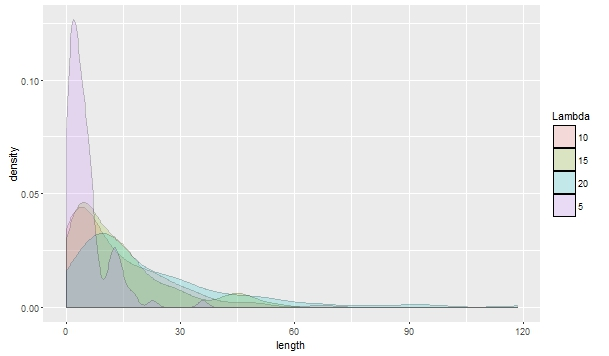
\includegraphics[width=1\linewidth]{Figuras/LAMBDAS}
\caption{Se graficaron distribuciones exponenciales con parámetro $\lambda=5, 10, 15, 20$}
\end{figure}

De aquí nace la siguiente pregunta: dada una observación $ X_0$, ¿cuál sería la $ \lambda_{i}$ que le asigne mayor probabilidad o densidad a la ocurrencia de esta observación? Por ejemplo, de la gráfica anterior se puede observar que si $x_{0}=5$, el mejor valor de lambda sería $\lambda=5$, mientras que si $x_{0}=30$, sería $\lambda=15$. Siguiendo la misma línea de pensamiento, también sería acertado preguntarse por el mejor estimador de $\beta$, donde la probabilidad de que ocurra $\lambda_{i}$ (que maximiza la la probabilidad de ocurrencia de $x_{0}$) sea máxima. Entonces, la función de verosimilitud para $X_{0}$ es:\\
\begin{equation*}
 Lik(\beta|X)=f_{x}(x)=\dfrac{\beta}{(x+\beta)^{2}}=\underset{0}{\overset{\infty }{\int }}f_{x|\lambda}(x)f(\lambda)d\lambda
\end{equation*}

 
Y con el planteamiento anterior, en lugar de buscar el mejor estimador de $\beta$ en Lik($\beta|X_{0}$), podríamos preguntarnos por la mejor $\lambda_{i}$ inducida por $\beta$ tal que $\beta$ maximice la ocurrencia de $\lambda_{i}$, y a su vez, $\lambda_{i}$ maximice la probabilidad de haber observado  $X_{0}$. Entonces con este enfoque, la función de verosimilitud para $X_{0}$ queda expresada de la siguiente manera:

\begin{equation*}
Lik(\lambda_{i},\beta|X_{0})=f_{x|\lambda_{i}}(x|\beta,\lambda_{i})f(\lambda{i})
\end{equation*}
	
	Siguiendo las ideas planteadas previamente, la verosimilitud extendida se define de la siguiente forma:\\
	
	Sean ${X}_{i=1}^{n}$ un conjunto de vectores aleatorios independientes e idénticamente distribuidos de dimensión p con algún vector de parámetros $\theta$, y sea $u$ una variable aleatoria con algún vector de parámetros $\beta$ y con soporte en $R_{+}$, tal que $X_{i}$ se puede esxpresar como una distribución tipo mezcla con variable de mezcla $u$. Entonces  $f_{X_{i}}(x_{i})=\underset{0}{\overset{\infty }{\int }}f_{x_{i}|u}(x_{i})f_{u}(u)du$ para toda $i$, con $X_{i}$ dado $u_{i}$ condicionalmente independiente a $X_{j}$ dado $u_{j}$, y $ u_{i}$ dado $\beta$ independiente a $u_{j}$ dado $\beta$ para toda $i$ diferente de $j$, por lo que la verosimilitud extendida es:\\
	\begin{equation*}
	Lik(u_{i},\theta,\beta |X)=\prod_{i=1}^{n}f_{x_{i}|u_{i}}(x|\theta, u_{i},\beta)f_{u_{i}}(u_{i}|\beta)
	\end{equation*}
	
	
	donde $u_{i}$ es una variable latente.\\
	
	Trabajar con la verosimilitud extendida podría parecer más complicado al tener que estimar una variable latente para cada observación de $X$, pero en ocasiones resulta más sencillo optimizar la función $\prod_{i=1}^{p}f_{x_{i}|u_{i}}(x_{i})f(u_{i})$ que $f(X)$ y, además, existen algoritmos computacionales, vía cadenas de Markov, o el algoritmo EM, que permiten encontrar los estimadores de los parámetros deseados. Por lo qué ahora se hablará brevemente de los distintos y posible métodos a implementar.

%\begin{algorithm}[H]
%	\SetAlgoLined
%	\KwResult{Write here the result }
%	initialization\;
%	\While{While condition}{
%		instructions\;
%		\eIf{condition}{
%			instructions1\;
%			instructions2\;
%		}{
%		instructions3\;
%	}
%}
%\caption{How to write algorithms}
%\end{algorithm}


\subsection{Muestreador de Gibbs}
El muestreador de Gibbs es un método de simulación tipo Markov Chain Montecarlo (MCM), estos métodos permiten obtener muestras de alguna densidad de probabilidad $f_{x}$ mediante la construcción de una cadena de Markov que converga a dicha densidad.\\ 

El muestreador de Gibbs permite obtener una muestra de una distribución conjunta a partir de las distribuciones marginales, por lo que no es necesario conocer la distribución conjunta, basta con construir una cadena de Markov adecuada  con las distribuciones marginales, las cuales convergerán a una muestra aleatoria de la distribución conjunta.\\

De forma intuitiva, el muestreador de Gibbs se plantea de la siguiente manera; supongamos que tenemos una distribución de la forma $f(X,\Theta)$ donde X es un vector aleatorio y $\Theta$ algún vector de parámetors del cual se desearía tener una muestra mediante una cadena de Markov, es decir, obtener una muestra de $f(\theta ^{k}|X)$ a partir de una sucesión de parámetros ${\theta}_{k=1} ^{\infty}$, tal que la probabilidad de transición de esta sucesión converja a la distribución de la cual se desearía tener una muestra, esto es, $\lim_{k->\infty} P(\theta^{k+1}|\theta^{k},X)=P(\theta|X)$. Dada la descripción del modelo anterior, la cadena debe ser estacionaria, irreducible, aperiódica y recurrente positiva. La propiedad de estacionariedad asegurar que $P(\theta|X)$ no cambie cuando $k$ tienda a infinito; irreducible para no descartar ningún valor posible de $\theta ^{k}$ en cada iteración; mientras que, aperiodicidad para que la cadena no tenga ciclos, y así permanecer en el estado estacionario. Por último, recurrente positiva, para que se pueda visitar cualquier estado un número infinito de veces y así asegurar que la distribución límite tomó toda la información disponible en consideración.\\

Ahora bien, para encontrar una cadena que nos permita obtener las caractrísticas anteriores German $\&$ German (citar bien esta parte) demuestra que  $ \lim_{k->\infty} P(\theta^{k}|X)=P(\theta|X)$, donde:
 
 \begin{equation*}
 P(\theta^{k}|X)=\stackrel{~}{{\prod}_{j=1}^{t }}P(\theta_{j}|X,...,\theta_{j-1},\theta_{j+1},...,\theta_{n}) 
 \end{equation*}

 y $\theta_{j}$ dado $X,...,\theta_{j-1},\theta_{j+1},...,\theta_{n}$ es condicionalmente independiente para toda $j$, para alguna medida de probabilidad arbitraria $P(.)$. Entonces si $\theta_{j} ^{k}$ se distribuye $ f(\theta_{j} ^{k}|X,...,\theta_{j-1},\theta_{j+1},...,\theta_{n})$, de aquí se puede obtener facilmente una muestra de $\theta_{j} ^{k}$ para toda $j$, si su densidad tiene una forma cerrada, y así se construiría una cadena de Markov con las caractarísticas deseadas, $[\theta^{k}] _{1} ^{\infty}$, con probabilidad de transición $P(\theta^{k}|X)$.\\

Entonces los pasos para implementar el Muestreador de Gibbs son los siguientes:\\

Dar un conjunto de valores iniciales $\Theta_{0}$, no importa cuáles valores se den, la propiedad de estacionareidad, asegurará la convergencia al estado estacionario. El vector $\theta$ puede ser particionado en d subconjuntos excluyentes, tal que d$<=$n, con la finalidad de simplificar los cálculos. Convenientemente se pueden seleccionar los sobconjuntos de modo que los que tienen alta correlación queden juntos.\\

Para cada $\theta_{j}$ obtener su distribución condicionada \begin{equation*}
f(\theta_{j} |X,...,\theta_{0,j-1},\theta_{0,j+1},...,\theta_{0,n})
\end{equation*} y realizar una simulación de esta. El valor de $\theta_{j}$ obtenido reemplazará a los valores iniciales. En caso de que no se pueda tener la distribución de $\theta|_{X,\theta \ \theta_{j}}$ se realiza un procedimiento de aceptación-rechazo para obtener una realización de $\theta_{j}$.\\

Una vez obtenidos todos los valores de $\theta|_{X,\theta, \ \theta_{j}}$ se reemplazan por los valores iniciales y se repite el procedimiento hasta que la cadena se estabilice.

Computacionalmente el algoritmo se vería de la siguiente forma:\\


%\lstinputlisting[language=R]{h.r}
%\begin{algorithmic}
%	\caption{Muestreador de Gibbs}\label{alg:gibbs}
%	\begin{algorithmic}[1]
%		\Procedure{$\Theta_{k} <- (\theta_{1,0},...,\theta_{d,0})$}{}\Comment{Conjunto de valores iniciales.}
%		\State $r\gets a\bmod b$
%		\For{$r\not=0$}\Comment{We have the answer if r is 0}
%		\State $a\gets b$
%		\State $b\gets r$
%		\State $r\gets a\bmod b$
%		\EndWhile\label{euclidendwhile}
%		\State \textbf{return} $b$\Comment{The gcd is b}
%		\EndProcedure
%	\end{algorithmic}
%\end{algorithmic}


\begin{center}
	$\Theta_{k} <- (\theta_{1,0},...,\theta_{d,0})$\\
	$M<-$ número total de iteraciones.\\
	for $k < M$ \\
		
			$\theta_{j} ^{k+1}<-$ random ($\Pi$($\theta|_{X,\theta^{k} \ \theta_{j} ^{k}}$))\\
		              
	end for\\
\end{center}
									

\section{Algoritmo para la distribución hiperbólica generalizada}

Supongamos que tenemos una colección de $r_{n}$ datos, donde cada $r_{i}\in R^{p}$, de los cuales tenemos motivos para creer que fueron generados por una distribución hiperbólica generalizada p-variada. Entonces nos interesaría inferir los valores de los parámetros de dicha distribución, pero antes de ello sería conveniente expresar a nuestra distribución de interés como una distribución tipo mezcla normal, con variable de mezcla $u$ con distribución Gaussiana inversa (GI), por lo que así podemos replantear el problema, enfocándonos en buscar los parámetros de la distribución de mezcla, $\mu,\beta,\Sigma$.\\

Ahora con un enfoque bayesiano, podemos plantear la verosimilitud de la distribución \textit{aposteriori} de $\mu,\beta,\Sigma$, es decir:
\begin{equation*}
f(\mu,\beta,\Sigma|(r_{i})_{i=1}^{n})=\prod_{i=1}^{n}f_{r_{i}}(r_{i}|\mu,\beta,\Sigma)\Pi(\mu,\beta,\Sigma)
\end{equation*}   
Donde $\Pi(\mu,\beta,\Sigma)$ es la distribución conjunta a \textit{apriori} de $\mu,\beta$ y $\Sigma$, y además asumiremos que tanto $\mu,\beta,\Sigma$ son independientes, por lo que:
\begin{equation*}
f(\mu,\beta,\Sigma|(r_{i})_{i=1}^{n})=\prod_{i=1}^{n}f_{r_{i}}(r_{i}|\mu,\beta,\Sigma)\Pi(\mu|\mu_{0},\Sigma_{0})\Pi(\beta|\mu_{\beta},\Sigma_{\beta})\Pi(\Sigma|S)
\end{equation*}
 Como supuesto adicional, asumiremos que $\mu$ se distribuye $N(\mu_{0},\Sigma_{0})$, $\beta$ se distribuye $N(\beta_{0},\Sigma_{\beta})$, y $\Sigma$ se distribuye $W^{-1}(S,n,p)$. Así, nuestra función de verosimilitud adquiere la siguiente forma:
\begin{equation*}
Lik(\mu,\mu_{0},\beta,\beta_{0},\Sigma,\Sigma_{0},\Sigma_{\beta},S|(r_{i})_{i=1}^{n})=
\end{equation*}
Luego, expresando a nuestra distribución de interés $f_{r_{i}}(r_{i})$ como una distribución tipo mezcla normal, con variable de mezcla $u$, la función de verosimilitud tiene la sigueinte forma:
 
\begin{equation*}
\prod_{i=1}^{n}\int_{0}^{\infty}N_{p}(r_{i}|\mu,u\beta,u\Sigma)GI(u|\lambda_{0},\Psi_{0})g(\mu,\beta,\Sigma)du,
\end{equation*}
donde $g(\mu,\beta,\Sigma)=N_{p}(\mu|\mu_{0},\Sigma_{0})N_{p}(\beta|\beta_{0},\Sigma_{\beta})W_{pxp}(\Sigma|S)$

Por lo que ahora necesitamos conocer también los valores de $\lambda$ y $\Psi$ propios de la distribución gaussiana inversa, para ello supondremos que $\lambda$ y $\psi$ son independientes, y además gracias a la gran flexibilidad de la distribución gamma, asumiremos que cada uno de ellos proviene de una distribución gamma con parámetros $\alpha_{\lambda}$, $\beta_{\lambda}$, $\alpha_{\Psi}$ y $\beta_{\Psi}$, respectivamente, por lo que la distribución \textit{apriori} para $\lambda$ y $\Psi$ está dada de la siguiente manera:

\begin{equation*}
\Pi(\lambda,\Psi)=\Pi(\lambda|\alpha_{\lambda},\beta_{\lambda})\Pi(\Psi|\alpha_{\Psi},\beta_{\Psi})
\end{equation*}

Ahora según lo expuesto en el capítulo 3.algo, es conveniente extender la verosimilitud; esto es que:
\begin{equation*}
Lik(\mu,\beta,\Sigma,(u_{i})_{i=1}^{n},\lambda,\Psi|(r_{i})_{i=1}^{n},\mu_{0},\beta_{0},\Sigma_{\mu},\Sigma_{\beta},S,\alpha_{\lambda},\beta_{\lambda},\alpha_{\Psi},\beta_{\Psi})=
\end{equation*}
\begin{equation*}
\prod_{i=1}^{n}N_{p}(r_{i}|\mu,u_{i}\beta,u_{i}\Sigma)GI(u_{i}|\lambda_{0},\Psi_{0})\Pi(\lambda|\alpha_{\lambda},\beta_{\lambda})\Pi(\Psi|\alpha_{\Psi},\beta_{\Psi}) 
\end{equation*}
\begin{equation*}
N_{p}(\mu|\mu_{0},\Sigma_{0})N_{p}(\beta|\mu_{\beta},\Sigma_{\beta})W^{-1}_{pxp}(\Sigma|S,n,p)
\end{equation*}
Una vez teniendo nuestra función de verosimilitud, ya estamos en condiciones de proponer algún método numérico para encontrar los parámetros de interés; para ello, por un lado se utilizará el muestreador de GIBBS para obtener una muestra de los parámetros buscados; por otro lado se optará por un enfoque bayesiano para tratar la verosimilitud, ya que gracias a este método, podemos aprovechar la información implícita de los datos.\\

Entonces, con un enfoque bayesiano, será necesario encontrar las distribuciones marginales de los parámetros de interés, para que una vez obtenidas se pueda implementar el muestreador de GIBBS.\\ 


Por lo que ahora necesitamos conocer las distribuciones marginales de:
\begin{eqnarray*}
& &\Pi(\mu|\beta,\Sigma,(u_{i})_{i=1}^{n},\lambda,\Psi,(r_{i})_{i=1}^{n},\mu_{0},\beta_{0},\Sigma_{\mu},\Sigma_{\beta},S,\alpha_{\lambda},\beta_{\lambda},\alpha_{\Psi},\beta_{\Psi}) \\
& & \Pi(\beta|\mu,\Sigma,(u_{i})_{i=1}^{n},\lambda,\Psi,(r_{i})_{i=1}^{n},\mu_{0},\beta_{0},\Sigma_{\mu},\Sigma_{\beta},S,\alpha_{\lambda},\beta_{\lambda},\alpha_{\Psi},\beta_{\Psi}) \\
& &\Pi(\Sigma|\mu,\beta,(u_{i})_{i=1}^{n},\lambda,\Psi,(r_{i})_{i=1}^{n},\mu_{0},\beta_{0},\Sigma_{\mu},\Sigma_{\beta},S,\alpha_{\lambda},\beta_{\lambda},\alpha_{\Psi},\beta_{\Psi}) \\
& & \Pi(u_{i}|\mu,\beta,\Sigma,\lambda,\Psi,(r_{i})_{i=1}^{n},\mu_{0},\beta_{0},\Sigma_{\mu},\Sigma_{\beta},S,\alpha_{\lambda},\beta_{\lambda},\alpha_{\Psi},\beta_{\Psi})\\
& & \Pi(\lambda|\mu,\beta,\Sigma,(u_{i})_{i=1}^{n},\Psi,(r_{i})_{i=1}^{n},\mu_{0},\beta_{0},\Sigma_{\mu},\Sigma_{\beta},S,\alpha_{\lambda},\beta_{\lambda},\alpha_{\Psi},\beta_{\Psi}) \\
& &\Pi(\Psi|\mu,\beta,\Sigma,(u_{i})_{i=1}^{n},\lambda,(r_{i})_{i=1}^{n},\mu_{0},\beta_{0},\Sigma_{\mu},\Sigma_{\beta},S,\alpha_{\lambda},\beta_{\lambda},\alpha_{\Psi},\beta_{\Psi})\\
\end{eqnarray*}




%\begin{equation*}
%\Pi(\mu|\beta,\Sigma,(u_{i})_{i=1}^{n},\lambda,\Psi,(r_{i})_{i=1}^{n},\mu_{0},\beta_{0},\Sigma_{\mu},\Sigma_{\beta},S,\alpha_{\lambda},\beta_{\lambda},\alpha_{\Psi},\beta_{\Psi}) 
%\end{equation*}
%\begin{equation*}
%\Pi(\beta|\mu,\Sigma,(u_{i})_{i=1}^{n},\lambda,\Psi,(r_{i})_{i=1}^{n},\mu_{0},\beta_{0},\Sigma_{\mu},\Sigma_{\beta},S,\alpha_{\lambda},\beta_{\lambda},\alpha_{\Psi},\beta_{\Psi}) 
%\end{equation*}
%\begin{equation*}
%\Pi(\Sigma|\mu,\beta,(u_{i})_{i=1}^{n},\lambda,\Psi,(r_{i})_{i=1}^{n},\mu_{0},\beta_{0},\Sigma_{\mu},\Sigma_{\beta},S,\alpha_{\lambda},\beta_{\lambda},\alpha_{\Psi},\beta_{\Psi}) 
%\end{equation*}
%\begin{equation*}
%\Pi(u_{i}|\mu,\beta,\Sigma,\lambda,\Psi,(r_{i})_{i=1}^{n},\mu_{0},\beta_{0},\Sigma_{\mu},\Sigma_{\beta},S,\alpha_{\lambda},\beta_{\lambda},\alpha_{\Psi},\beta_{\Psi})
%\end{equation*}
%\begin{equation*}
%\Pi(\lambda|\mu,\beta,\Sigma,(u_{i})_{i=1}^{n},\Psi,(r_{i})_{i=1}^{n},\mu_{0},\beta_{0},\Sigma_{\mu},\Sigma_{\beta},S,\alpha_{\lambda},\beta_{\lambda},\alpha_{\Psi},\beta_{\Psi}) 
%\end{equation*}
%\begin{equation*}
%\Pi(\Psi|\mu,\beta,\Sigma,(u_{i})_{i=1}^{n},\lambda,(r_{i})_{i=1}^{n},\mu_{0},\beta_{0},\Sigma_{\mu},\Sigma_{\beta},S,\alpha_{\lambda},\beta_{\lambda},\alpha_{\Psi},\beta_{\Psi}) 
%\end{equation*}


\section{Distribuciones marginales completas}

\subsection{Para $\mu$}
Para encontrar la distribución marginal de $\mu|\beta,\Sigma,(u_{i})_{i=1}^{n},(r_{i})_{i=1}^{n}$ a partir de la función de verosimilitud, podemos tomar las densidades donde aparece $\mu$ e identificar su kernel, es decir, de: 

\begin{eqnarray*}
& &\prod_{i=0}^{n}N_{p}(r_{i}|\mu,u_{i}\beta,u_{i}\Sigma)N_{p}(\mu|\mu_{0},\Sigma_{0})=
 \\
& & \prod_{i=1}^{n}\dfrac{exp(-\frac{1}{2}(r_{i}-\mu-u_{i}\beta)'(u_{i}\Sigma)^{-1}(r_{i}-\mu-u_{i}\beta))}{(2u_{i}\Pi)^{p/2}|\Sigma|^{1/2}}\\
& & \dfrac{exp(-\frac{1}{2}(\mu-\mu_{0})'\Sigma_{0}(\mu-\mu_{0}))}{(2\Pi)^{p/2}|\Sigma|^{1/2}}\\
\end{eqnarray*}
%\begin{equation*}
%\prod_{i=0}^{n}N_{p}(r_{i}|\mu,u_{i}\beta,u_{i}%\Sigma)N_{p}(\mu|\mu_{0},\Sigma_{0})=
%\end{equation*}
%\begin{equation*}
%\prod_{i=1}^{n}\dfrac{exp(-\frac{1}{2}(r_{i}-\mu-u_{i}\beta)'(u_{i}\Sigma)^{-1}(r_{i}-\mu-u_{i}\beta))}{(2u_{i}\Pi)^{p/2}|\Sigma|^{1/2}}\dfrac{exp(-\frac{1}{2}(\mu-\mu_{0})'\Sigma_{0}(\mu-\mu_{0}))}{(2\Pi)^{p/2}|\Sigma|^{1/2}}
%\end{equation*}

tomando el cambio de variable  $r_{i}\acute{}=r_{i}-u_{i}\beta$, nos quedamos con:
 \begin{equation*}
 \prod_{i=1}^{n}exp(-\frac{1}{2}(\mu-r_{i}')'(u_{i}\Sigma)^{-1}(\mu-r_{i}'))exp(-\dfrac{1}{2}(\mu-\mu_{0})'\Sigma_{0}(\mu-\mu_{0}))
 \end{equation*}
Después, trabajando únicamente con:
\begin{eqnarray*}
& &\prod_{i=1}^{n}exp(-\frac{1}{2}(\mu-r_{i}')'(u_{i}\Sigma)^{-1}(\mu-r_{i}'))=
 \\
& & exp(-\frac{1}{2}\sum_{i=1}^{n}(\mu-r_{i}')'(u_{i}\Sigma)^{-1}(\mu-r_{i}')) = \\
& &exp(-\frac{1}{2}\sum_{i=1}^{n}(\mu'(u_{i}\Sigma)^{-1}\mu  -2\mu(u_{i}\Sigma)^{-1}r_{i}' -r_{i}'(u_{i}\Sigma)^{-1}r_{i}' )\alpha 
 \\
& &  exp(-\frac{1}{2}\sum_{i=1}^{n}(\mu'(u_{i}\Sigma)^{-1}\mu  -2\mu(u_{i}\Sigma)^{-1}r_{i}')= \\
& & 
exp(-\frac{1}{2}(\mu'(U\Sigma)^{-1}\mu  -2\mu(U\Sigma)^{-1}R), \\
\end{eqnarray*}
donde : 

\begin{equation*}
U=(\sum_{i=1}^{n}\dfrac{1}{u_{i}})^{-1}, R= \sum_{i=1}^{n}\dfrac{r_{i}}{u_{i}}U
\end{equation*}
Entonces, según el anexo 4, a esta parte del kernel de $\mu$ le corresponda una distribución normal p variada con vector de medias $R$, y matriz de varianza covarianza $U\Sigma$. Luego, multiplicando el Kernel anterior por la densidad de $\mu$, y por el anexo 6, se tiene que $\mu$ se distribuye normal con vector de medias:
\begin{equation*}
(R(U\Sigma)^{-1}+\mu_{0}\Sigma_{0}^{-1})(U\Sigma^{-1}+\Sigma_{0}^{-1})^{-1}
\end{equation*}
 y matriz de varianza covarianza:
 \begin{equation*}
 U\Sigma+\Sigma_{0}
 \end{equation*}

\subsection{Para $\beta$}
Mediante un procedimiento similar, encontraremos el Kernel de $\beta$ dado las demás variables de interés. Entonces, de la función de verosimilitud, nos quedamos con la parte donde sólo aparece $\beta$, es decir:
\begin{equation*}
\prod_{i=0}^{n}N_{p}(r_{i}|\mu,u_{i}\beta,u_{i}\Sigma)N_{p}(\beta|\mu_{\beta},\Sigma_{\beta})
\end{equation*}
Luego trabajando con el producto de las n variables normales p variadas correspondientes a $r_{i}$,  considerando los términos que únicamente dependen de $\beta$, y con el cambio de variable $\mu_{i}=r_{i}-\beta$, tenemos que:
\begin{equation*}
\prod_{i=1}^{n}exp(-\dfrac{1}{2}(r_{i}-\mu-u_{i}\beta)'(u_{i}\Sigma)^{-1}(r_{i}-\mu-u_{i}\beta))=
\end{equation*}
\begin{equation*}
exp(-\frac{1}{2}\sum_{i=1}^{n}((u_{i}\beta-\mu_{i})'(u_{i}\Sigma)^{-1}(u_{i}\beta-\mu_{i}))
\end{equation*}

Nuevamente desarrollando el exponente de la función exponencial, y quedándonos únicamente con la parte que depende de $\beta$ tenemos que:
\begin{equation*}
exp(-\dfrac{1}{2}\sum_{i=1}^{n}((u_{i}\beta)'(u_{i}\Sigma)^{-1}(u_{i}\beta)-2(u_{i}\beta)'(u_{i}\Sigma)^{-1}\mu_{i}))=
\end{equation*}
\begin{equation*}
exp(-\dfrac{1}{2}(\beta(V\Sigma)^{-1}\beta-2\beta(V\Sigma)^{-1}VM)
\end{equation*}
Donde:
\begin{equation*}
V=\frac{1}{\sum_{i=1}^{n}u_{i}} , M=\sum_{i=1}^{n}(r_{i}-\mu)
\end{equation*}
 Por lo tanto, según el anexo 4, el Kernel del producto de las n variables normales p-variadas correspondientes a $\beta$ corresponde a una distribución Normal con vector de medias $VM$, y matriz de varianza covarianza $V\Sigma$.
Luego, según el anexo 6, juntando el Kernel obtenido anteriormente con la densidad de $\beta$, se tiene que $\beta$ se distribuye normal p variado con vector de medias: 
\begin{equation*}
(MV\Sigma)^{-1}+\mu_{\beta}'\Sigma_{\beta}^{-1})((V\Sigma)^{-1}+\Sigma_{\beta}^{-1})^{-1}
\end{equation*}
Y matriz de varianza covarianza:
\begin{equation*}
V\Sigma+\Sigma_{\beta}
\end{equation*}

\subsection{Para $\Sigma$}
Para encontrar la distribción marginal de $\Sigma$ a partir de la función de verosmilitud, podemos tomar las densidades donde aparece $\sigma$, y a partir de ahí, identificar el Kernel correspondiente, es decir, tomando: 
\begin{equation*}
\prod_{i=0}^{n}N_{p}(r_{i}|\mu,u_{i}\beta,u_{i}\Sigma)W^{-1}_{pxp}(\Sigma|S,n,p)
\end{equation*}
Y luego trabajando con el producto de las n variables normales p-variadas correspondientes a $r_{i}$, considerando los términos que únicamente dependen de $\Sigma$, y con el cambio de variable $(x_{i}=r_{i}-\mu-\beta)/\sqrt{u_{i}}$, tenemos que:
\begin{eqnarray*}
& &\prod_{i=1}^{n}exp(-\dfrac{1}{2}(r_{i}-\mu-u_{i}\beta)'(u_{i}\Sigma)^{-1}(r_{i}-\mu-u_{i}\beta))\\
& &\dfrac{\exp(-\frac{1}{2}tr(\Sigma^{-1}S))}{|\Sigma|^{n/2}}\\
& =&\dfrac{\exp(-\frac{1}{2}\sum_{i=1}^{n}x_{i}\Sigma^{-1}\sum_{i=1}^{n}x_{i})}{|\Sigma|^{\frac{n}{2}}}\dfrac{\exp(-\frac{1}{2}tr(\Sigma^{-1}S))}{|\Sigma|^{\frac{n}{2}}}
 \\
& =&\dfrac{\exp(-\frac{1}{2}(X\Sigma^{-1}X + tr(\Sigma^{-1}S)))}{|\Sigma|^{n}} \\
& =&\dfrac{\exp(-\frac{1}{2}(tr(\Sigma^{-1}XX') + tr(\Sigma^{-1}S))))}{|\Sigma|^{n}}
 \\
& =&\dfrac{\exp(-\frac{1}{2}(tr(\Sigma^{-1}(XX' + S))))}{|\Sigma|^{n}}
 \\
\end{eqnarray*}

Haciendo $X=\sum_{i=1}^{n}x_{i}$, y ya que $X\Sigma^{-1}X=tr(\Sigma^{-1}(XX')) $. La última expresión corresponde al kernel de una distribución Whishart con matriz de escala $XX'+ S$, y $2n$ grados de libertad.
\section{Para $\lambda$}
Para encontrar la distribción marginal de $\lambda$ a partir de la función de verosmilitud, podemos tomar las densidades donde aparece $\lambda$, y a partir de ahí, identificar el Kernel correspondiente; es decir, de la sigueinte expresión:
\begin{equation*}
\prod_{i=1}^{n}GI(u_{i}|\lambda,\Psi)\Pi(\lambda|\alpha_{\lambda},\beta_{\lambda})
\end{equation*}
nos quedamos con:
\begin{equation*}
\prod_{i=1}^{n}\sqrt{\lambda}\exp(-\frac{\lambda(u_{i}-\Psi)^{2}}{2\Psi^{2}u_{i}}\lambda^{\beta_{\lambda}-1}\exp(-\lambda\alpha_{\lambda})\alpha
\end{equation*}
\begin{equation*}
\lambda^{n/2+\beta_{\lambda} -1}\exp(-X\lambda)
\end{equation*}
donde $X=\sum_{i=1}^{n}\dfrac{(u_{i}-\Psi)^{2}}{2\Psi^{2}u_{i}} - \alpha_{\lambda}$.
Por lo que tenemos que el kernel correponde a una distribución gamma, concluimos que $\lambda$ se distribuye gamma con parámetros $(\frac{n}{2}+\beta_{\lambda}),X$.

\section{Para $\Psi$}
Para encontrar la distribción marginal de $\Psi$ a partir de la función de verosmilitud, podemos tomar las densidades donde aparece $\Psi$, y a partir de ahí identificar el Kernel correspondiente; es decir, de la sigueinte expresión:
\begin{equation*}
	\prod_{i=1}^{n}GI(u_{i}|\lambda,\Psi)\Pi(\Psi|\alpha_{\Psi},\beta_{\Psi})
\end{equation*}
nos quedamos con:
\begin{equation*}
	\prod_{i=1}^{n}\sqrt{\lambda}\exp(-\frac{\lambda(u_{i}-\Psi)^{2}}{2\Psi^{2}u_{i}})\Psi^{\beta_{\Psi}-1}\exp(-\Psi\alpha_{\Psi}) \alpha
\end{equation*}
\begin{equation*}
\exp(-\sum_{i=1}^{n}\frac{\lambda(u_{i}-\Psi)^{2}}{2\Psi^{2}u_{i}})\Psi^{\beta_{\Psi}-1}\exp(-\Psi\alpha_{\Psi}) \alpha
\end{equation*}
\\
El Kernel obtenido resulta difícil de identificar, y tal vez sea complicado obtener la densidad condicional  de $\Psi$, necesaria para implementar el muestreador de GIBBS; por lo que se atacará este problema por medio de una herramienta útil en simulación, llamada slice sampler; la ventaja de utilizar el slice sampler es que nos permite obtener una muestra aleatoria de algúna distribución de probabilidad, con tan solo conocer su Kernel.


\section{Para $u_{i}$}
Para encontrar la distribción marginal de $u_{i}$ a partir de la función de verosmilitud, podemos tomar las densidades donde aparece $u_{i}$, y a partir de ahí identificar el Kernel correspondiente, es decir, de la sigueinte expresión:

\begin{equation*}
\prod_{i=1}^{n}N_{p}(r_{i}|\mu,u_{i}\beta,u_{i}\Sigma)GI(u_{i}|\lambda,\Psi)
\end{equation*}

nos quedamos con:

\begin{eqnarray*}
& &\dfrac{exp(-\frac{1}{2}(r_{i}-\mu-u_{i}\beta)'(u_{i}\Sigma)^{-1}(r_{i}-\mu-u_{i}\beta))}{(u_{i})^{p/2}}\sqrt{\dfrac{1}{u_{i} ^{3}}} \\
& & \exp(-\dfrac{\lambda(u_{i}-\Psi)^{2}}{2\Psi^{2}u_{i}})
 \\
\end{eqnarray*}

EL kernel anterior parece muy difícil de identificar, e intentar encontrar la forma analítica de la distribución condicionada de $u_{i}$ puede resultar muy difícil, si no es que imposible, por lo que optaremos por obtener una muestra aleatoria de $u_{i}$ por medio del slice sampler.\\
Una vez descrita la metodología a emplear para inferir los parámetros de nuesta muestra de interés, ya estamos en condiciones de programar el muestreador de GIBBS y emplearlo para estudiar un conjunto de datos, lo cual se llevará acabo en el siguiente capítulo.




%	Bibliografia
\medskip
\addcontentsline{toc}{chapter}{Bibliograf\'ia}
\bibliography{tesis_davidcastillo_bibliografia}


%	Apendices
\appendix
	
\chapter{Estimación por máxima verosimilitud}
El método de máxima verosimilitud tiene un enfoque frecuentista, en el que los datos son generados por una función de densidad de probabilidad $f_{x}$, con la cual 
es posible construir una función de verosimilitud, la cual tiene como argumento los parámetros a estimar, y a su vez depende de los datos ya observados. Por lo regular la función de verosimilitud se construye de acuerdo al evento, concerniente a los datos de interés, por lo que muchas veces es la misma función de densidad, pues se considera el evento en que la variable aleatoria $X_{i}$ tome el valor $x_{i}$. De manera intuitiva, la función de verosimilitud representa la probabilidad de haber observado la variable aleatoria $X$ bajo el modelo dado, la cual se pretende maximizar con respecto al parámetro de interés para así obtener qué tan probable es que el modelo dado haya generado los datos.

En términos generales los estimadores máximo verosimiles se construyen de la siguiente forma:
\begin{enumerate}
	\item Construir la función de verosimilitud, la cual llamaremos $LIK(\Theta|X)$
	\item Plantear el problema de maximización:  
\begin{equation*}
max_{\Theta}(LIK(\Theta|X))
\end{equation*} 
\item La solucion $\Theta *$ del problema de maximización es el estimador buscado.
\end{enumerate}

Aunque el algoritmo para encontrar estimadores máximo verosimiles parece sencillo, no siempre lo es, pues la dificultad del proceso de maximización aumenta conforme más variables se tienen, lo cual puede llevar a procesos computacionales poco eficientes. Estas dificultades incentiva el uso del algoritmo EM.

	\chapter{Algoritmo EM}
El algoritmo Expectation Maximization (EM) fue formalizado por Dempster
et al (1977); este algoritmo tiene un enfoque frecuentista, y tiene como objetivo encontrar los estimadores máximo verosímiles de funciones de densidad con datos no observados, lo cual es ideal para manejar distribuciones tipo mezcla, pues la variable de mezcla toma el lugar de los datos no observados.  

Para implementar el algoritmo EM se requiere un conjunto de datos u observaciones $x_{i}$, de las cuales se conoce su función paramétrica de densidad; el parámetro de dicha distribución, $\Theta$, es desconocido y es lo que se pretende estimar; también se requiere la distribución, parametrizada por $\Theta$, de los datos no observados y finalmente una suposición inicial, $\Theta^{0}$, sobre el parámetro $\Theta$. 

De manera intuitiva, el algorimo EM se desarrolla de la siguiente forma:llamemos a la función de densidad asociada a $x_{i}$ como $f(x_{i}|\Theta)$, después supongamos que existen datos no observados $z$, y una función determinista $H(.)$ que tiene como dominio los datos no observados y como imagen los datos observados. Esto es, que para cada dato no observado se cumple que $H(Z_{s})=x_{i}$, para $Z_{s}$ un subconjunto de $Z$. Luego nos interesaría encontrar el valor de $\Theta$ que maximiza la probabilidad
de haber obtenido los datos no observados dado $\Theta$, pero justamente no conocemos los datos no observados $X$, por lo que la probabilidad anterior la ponderamos por la probabilidad de haber obtenido los datos no observados dados los datos sí observados y la suposición inicial del parámetro de interés, luego nos interesa maximizar $f(Z|\Theta ) f(Z|X,\Theta^{0})$, lo cual no nos libra del problema de los datos no observados. Entonces, nos fijamos en un promedio de todas las posibles posibilidades de $Z$, por lo que nuestra función a maximizar con respecto a $\Theta$ se convierte en:

\begin{equation*}
E_{Z}[f(Z|\Theta)]=\int_{Z}f(Z|\Theta)f(Z|X,\Theta^{0})dz
\end{equation*}

Por último, si se define a la esperanza descrita previamente como una función de $\Theta$, es decir, que $Q(\Theta|\Theta^{0})=E_{Z}[f(Z|\Theta)]$, entonces el problema planteado se resume en dado un valor $\Theta^{0}$, maximizar con respecto a $\Theta$ la función $Q(\Theta|\Theta^{0})$. De esta forma se crea un proceso iterativo, donde el valor $\Theta^{*}$ que maximiza la función $Q(.)$ se convierte ahora en $\Theta^{0}$, y el procedimiento se repite de nuevo; de esta forma se asegura que la esperanza converge a la verosimilitud buscada, y a su vez, $\Theta^{*}$ converge al estimador máximo verosímil. (citar dónde viene la demostración de esto)

En términos generales el estimador máximo verosimil a través del algoritmo EM se construye de la siguiente manera:

\begin{enumerate}
	\item Dar un valor inicial $\Theta^{0}$.
	\item Obtener las funciones de densidad $f(Z|\Theta)$, $f(Z|X,\Theta^{0})$.
	\item Calcular $Q(\Theta|\Theta^{0})=E_{Z}[f(Z|\Theta)]$, algunas veces resulta más sencillo calcular $E_{Z}[log(f(Z|\Theta))]$.
	\item Maximizar $Q(\Theta|\Theta^{0})$. 
	\item Una vez obtenido $\Theta^{*}$ sustituir por $\Theta^{0}$, y repetir los pasos $3$, $4$ y $5$, hasta que el algoritmo converja.
	 
\end{enumerate}

	\chapter{Slice sampler}

Los métodos de simulación slice sampler consisten en generar una cadena de Markov que converja a la distribución que se desea muestrear. La idea intuitiva de estos métodos consiste en suponer que el vector aleatorio bivariado $(X,Y)$ se distribuye uniforme en la región que está por debajo de la función de densidad, de la cual obtendríamos una muestra $(X_{0},Y_{0})$, y de está solo nos quedariamos con $X_{0}$, siendo esta nuestra variable de interés.\\ 

Ahora, para generar una muestra uniforme en dicha región, se utiliza un algoritmo recursivo con el fin de tener una cadena de markov que converja a la muestra deseada.\\

En términos ilustrativos el procedimiento es como sigue:\\

$1)$ Supongamos que tenemos el kernel o una densidad de una variable aleatoria univarada $X$, de la cual nos interesaría obtener una muestra aleatoria, y que además la gráfica de esta densidad es de la siguiente manera, por ejemlo:

\begin{figure}[h]
	\centering
	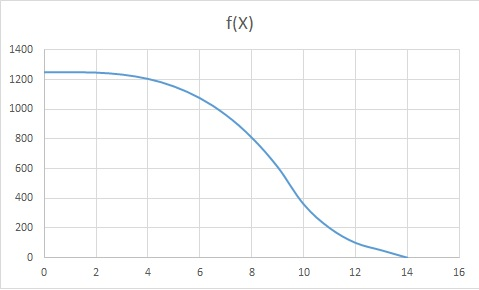
\includegraphics[width=0.7\linewidth]{Figuras/Slicesampler1}
	\caption{}
	\label{Grafica}
\end{figure}

\bigskip
$2)$ Luego definimos el vector aleatorio bivariado $(X,Y)$, el cual suponemos que se distribuye uniforme en la región que está por debajo de la gráfica anterior, y a esta región la denotamos como $U$, por lo que $U$ sería el conjunto de parejas $(x,y)$ con la propiedad de que $x$ es menor a $y$, siendo $y=f(x)$.\\ Entonces la región de la cual nos interesa obtener una muestra se ve de la siguiente forma:

\begin{figure}[h]
	\centering
	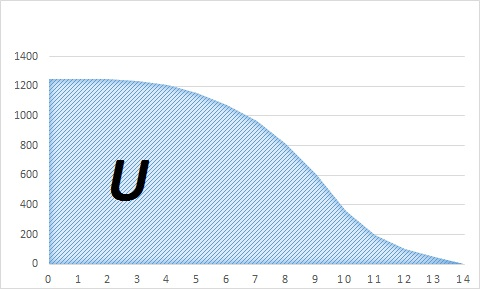
\includegraphics[width=0.7\linewidth]{Figuras/gs2}
	\caption{}
	\label{fig:gs2}
\end{figure}

\bigskip
$3)$ Ahora, proponemos un valor inicial $x_{0}$, y por el anexo (algo), si un vector aleatorio bivariado se distribuye uniforme en alguna región, entonces para cada valor que tome la variable $X$, la distribución marginal de $Y$ dado $X=x_{0}$ se distribuye uniforme dentro del segmento de recta $L(y)=((y,x_{0}) | y\in R)$, donde $L(y)$ está dentro de $U$. De esta manera, podríamos generar una realización de $Y$ dado $x_{0}$, así obtendríamos algún valor $y_{0}$, después fijamos éste valor $y_{0}$, y tendríamos ahora que $X$ dado $y_{0}$ se distribuye uniforme en $U\cap  L(x)=((x,y_{0})|x\in R)$, así obtendríamos una realización de $X$ dado $y_{0}$ de donde obtenríamos nuevamente un valor $x_{0}$. Así repetiriamos el proceso, pues de esta manera tenemos una cadena de Markov que converge a la realización de haber obtenido una muestra uniforme sobre $U$, donde sólo nos interesa el valor de $X$.\\
En la siguiente gráfica se ilustra el punto $3)$, por simplicidad se supuso que el primer valor que tomó la variable $X$ fue 0, luego $Y$ dado $x$ igual a cero se distribuye uniforme en el intervalo $(0,1200)$, de donde ahora obtenemos una realización de $Y$ dado $x$ igual a cero, donde Y tomó ahora el valor de $500$, con esta nueva información actualizamos el valor de $Y$, por lo que ahora obtenemos una realización de $X$ dado $Y$ igual a 500, y así seguimos actualizando los valores de $X$ y $Y$ hasta obtener la muestra deseada.

\begin{figure}[h]
	\centering
	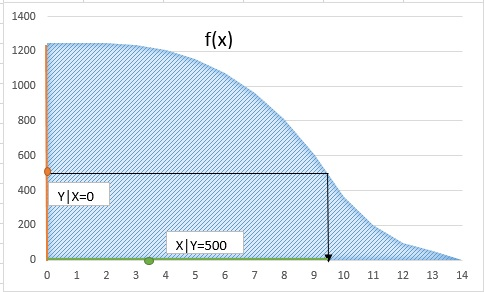
\includegraphics[width=0.7\linewidth]{Figuras/gs3}
	\caption{}
	\label{fig:gs3}
\end{figure}


	
\section{Simulación de distribuciones tipo mezcla normal en esperanza varianza}
Para generar distribuciones tipo mezcla normal en esperanza varianza basta con seguir los siguieentes pasos:

\begin{enumerate}
	\item Proponer valores para el vector de medias $\mu$, el vector de sesgo $\beta$, y la matriz de varianza-covarianza $\Sigma$.	
	\item Simular una realización de una variable aleatoria con soporte en los reales positivos, esta será nuestra variable de mezcla $u$.
	\item Realizar una simulación de $X$, donde $X$ se distribuye normal con vector de medias $\mu + u\beta$ y matriz de varianza-covarianza $\Sigma$.
	\item Realizar los pasos $2$) y $3$) hasta obtener la muestra deseada.
	 
\end{enumerate}
\section{Distribución tipo mezla normal p variada}
Se dice que el vector aleatorio $X\in R^{p}$ con densidad f(x) puede ser expresado como una distribución de mezcla normal $N(X|\mu,\beta,\Sigma)$ con variable de mezcla $u$ con densidad $f(u)$ y soporte en $R^{+}$, si:
\begin{equation*}
f(X|\mu,\beta,\Sigma)=\underset{0}{\overset{\infty }{\int }}N_{p}(X|\mu,u\beta,u\Sigma)f_{u}(u)du 
\end{equation*}

Donde, $N_{p}(X|\mu,u\beta,u\Sigma)$ es una distribución normal p-variada con vector de medias $\mu+u\beta$, y matriz de varianza-covarianza $u\Sigma$

\section{Covarianza de un vector aleatorio p variado}
Se define la covarianza de un vector aleatorio p variado como:
\begin{equation*}
COV(X)=E((X-\mu)(X-\mu)')
\end{equation*}
Siempre y cuando el vector de medias (del vector aleatorio $X$) $\mu$ exista.

\section{Covarianza de una distribución tipo mezcla}
Sea $X$ dado $u$ una distribución tipo mezcla de dimención p, y $u$ una variable de mezcla con soporte
en $R_{+}$, entonces la covarianza de $X$ se puede calcular como:
\begin{equation*}
COV(X)=E_{u}(COV(X|u))-COV_{u}(E(X|u))
\end{equation*}
Demostración:
De la definición de $COV(X)$ tenemos que:
\begin{eqnarray*}
COV(X)& = &E_{x}((X-\mu)(X-\mu)') \\
& =&E_{x}(XX'-2X\mu+\mu\mu')\\
& =&E_{x}(XX')-2E(X)\mu+\mu\mu' \\
& =&E_{x}(XX')-E_{x}(X)E_{x}(X)' \\
&= &E_{x}(XX')-E(X)_{x}E_{x}(X)'+E(X)_{x}E(X)_{x}'-\\
& &2E(X)_{x}E(X)_{x}'+E(X)_{x}E(X)_{x}\\
&= &E_{u}(E_{x}(XX'|u)-E_{x}(X|u)E_{x}(X|u)')+\\
& & E_{u}(E_{x}(X|u)E_{x}(X|u)') -2E_{u}(E_{x}(X|u)E(X)')\\
& & +E_{u}(E(X|u))E_{u}(E(X|U))\\
&= &E_{u}(E_{x}(XX'|u)-2E_{x}(X|u)E_{x}(x|u)'+
 \\
& &  E_{x}(X|u)E_{x}(X|u)') + E_{u}(E_(X|u)E_{x}(X|u)'\\
& & -2E_{x}(X|u)E_{u}(E_{x}(X|u))+\\
\end{eqnarray*}
\begin{eqnarray*}
& & E_{u}E_{x}(X|u)E_{u}E_{x}(X|u)') \\
&= &E_{u}(E_{x}(XX'-2XE_{x}(X|u)  \\
& & +E_{x}(X|u)E_{x}(X|U)) + \\
& & E_{u}((E_{x}(X|u)-E_{u}(E_{x}(X|u)))
\\
& & (E_{x}(X|u)-E_{u}(E_{x}(X|u)))')\\
&= &E_{u}((E_{x}(X)-E_{x}(X|u))(E_{x}(X)-E_{x}(X|u))') +  \\
& & COV_{u}(E_{x}(X|u))\\
& =&E_{u}(COV_{x}(X|u)) + COV_{u}(E_{x}(X|u)).
 \\
\end{eqnarray*}

\section{Kernel de una distribución normal p variada}
El kernel un vector aleatorio es la parte de la función de densidad que únicamente depende de dicho vector, y a su vez nos permite identificar de que familia proviene la distribución. Por ejemplo, en el caso de la distribución normal p variada
\begin{eqnarray*}
f(X|\mu,\Sigma)& =& \dfrac{1}{(2\Pi)^{p/2}|\Sigma|^{1/2}}\\
& &exp(-\dfrac{1}{2}(x'\Sigma^{-1}x - x'\Sigma^{-1}\mu -\mu'\Sigma^{-1}x+\mu'\Sigma^{-1}\mu))
 \\
\end{eqnarray*}

Tenemos que el Kernel correspondiente es:
\begin{equation*}
exp(-\dfrac{1}{2}(x'\Sigma^{-1}x -2x'\Sigma^{-1}\mu))
\end{equation*}
donde $\mu'\Sigma^{-1}x=x'\Sigma^{-1}\mu$, ya que es una forma cuadrática.

\section{Kernel de una distribución Wishart}
Análogamente al caso normal p variado, si nos concentramos en la parte de la densidad Wishart, con matriz de escala $S$ y con n grados de libertad, que únicamente depende de $\Sigma$, tenemos que el correspondiente kernel es:
\begin{equation*}
\dfrac{\exp(-\frac{1}{2}tr(\Sigma^{-1}S))}{|\Sigma|^{\frac{n}{2}}}
\end{equation*}

\section{Kernel del producto de n distribuciones normales p variadas con mismo vector de medias y misma matriz de varianza covarianza}
Supongamos que $X_{i}$ se distribuye normal p variada con vector de media $\mu$ y matriz de varianza covarianza $\Sigma$, entonces la función de  interés es de la siguiente manera:
\begin{equation*}
\prod_{i=1}^{n}N(X_{i}|\mu,\Sigma)=\prod_{i=1}^{n}\dfrac{1}{(2\Pi)^{p/2}|\Sigma|^{1/2}}exp(-\frac{1}{2}(X_{i}-\mu)'\Sigma^{-1}(X_{i}-\mu))
\end{equation*}
De aquí, trabajando únicamente con el exponente de la función exponencial tenemos que:
\begin{eqnarray*}
& &\prod_{i=1}^{n}exp(-\frac{1}{2}(X_{i}-\mu)'\Sigma^{-1}(X_{i}-\mu))= \\
& &exp(-\frac{1}{2}\sum_{i=1}^{n} (X_{i}-\mu)'\Sigma^{-1}(X_{i}-\mu))= \\
& &exp(-\dfrac{1}{2}\sum_{i=1}^{n}(X_{i}'\Sigma^{-1}X_{i}-2X_{i}'\Sigma^{-1}\mu+\mu'\Sigma^{-1}\mu))= \\
& &exp(-\frac{1}{2}(X'\Sigma^{-1}X-2X'\Sigma^{-1}\mu+n\mu\Sigma^{-1}\mu))
 \\
\end{eqnarray*}

Donde la jésima coordenada del vector X es $\sum_{i=1}^{n}X_{i,j}$
Por último,como sólo nos interesan los términos donde aparece $X_{i}$, llegamos a que el kernel es:
\begin{equation*}
exp(-\frac{1}{2}(X'\Sigma^{-1}X-2X'\Sigma^{-1}\mu))
\end{equation*} 

\section{Kernel del vector de medias de una distribución normal p variada multiplicada por la distribución del vector de medias}

En este caso tenemos que $X$ se ditribuye normal con vector de medias $\mu$ y matriz de varianza covarianza $\Sigma$, mientras que $\mu$ se distribuye normal con vector de medias $\mu_{0}$ y matriz de varianza covarianza $\Sigma_{0}$, y ahora nos interesa conocer el Kernel correspondiente a $\mu$, entonces tendríamos
que el producto de las funciones de densidad es:
\begin{equation*}
f_{X}(X|\mu,\Sigma)f_{\mu}(\mu|\mu_{0},\Sigma_{0})=    
\end{equation*}
\begin{equation*}
\dfrac{exp(-1/2(X-\mu)'\Sigma^{-1}(X-\mu))}{(2\Pi)^{p/2}|\Sigma|^{1/2}}       \dfrac{exp(-1/2(\mu-\mu_{0})'\Sigma_{0}^{-1}(\mu-\mu_{0}))}{(2\Pi)^{p/2}|\Sigma_{0}|^{1/2}}
\end{equation*}

Luego de cada función de densidad tomamos lo que dependa de $\mu$, para así obtener sus respectivos kerneles según el anexo 4,lo cual implica que:

\begin{eqnarray*}
& &Kernel = \\
& &exp(-\dfrac{1}{2}(\mu'\Sigma^{-1}\mu -2x'\Sigma^{-1}\mu))exp(-\dfrac{1}{2}(\mu'\Sigma_{0}^{-1}\mu -2\mu_{0}'\Sigma_{0}^{-1}\mu))=
 \\
& &exp(-\dfrac{1}{2}(\mu'\Sigma^{-1}\mu -2x'\Sigma^{-1}\mu + \mu'\Sigma_{0}^{-1}\mu -2\mu_{0}'\Sigma_{0}^{-1}\mu))=
 \\
& &exp(-\frac{1}{2}(\mu'(\Sigma^{-1}+\Sigma_{0}^{-1})\mu-2(X'\Sigma^{-1}+\mu_{0}'\Sigma_{0}^{-1})\mu)=
 \\
& &exp(-\frac{1}{2}(\mu'(\Sigma^{-1}+\Sigma_{0}^{-1})\mu-2(X'\Sigma^{-1}+\mu_{0}'\Sigma_{0}^{-1})(\Sigma^{-1}+\Sigma_{0}^{-1})^{-1} \\
& &(\Sigma^{-1}+\Sigma_{0}^{-1})\mu))
 \\
\end{eqnarray*}
De aquí se tiene que $\mu$ se distribuye normal p variada con matriz de varianza covarianza $\Sigma + \Sigma_{0}$, y vector de medias $(X'\Sigma^{-1}+\mu_{0}'\Sigma_{0}^{-1})(\Sigma^{-1}+\Sigma_{0}^{-1})^{-1}$

\section{Probabilidad condicional} \label{A.Ross}
La probabilidad condicional se define de la siguiente manera \cite{Ross_P}:

Si $P(F)>0)$, entonces:
\begin{equation*}
P(E\ F)=\frac{P(E\bigwedge F)}{P(F)}
\end{equation*}
	%\chapter{Pruebas de multinormalidad}
Para rechazar la hipótesis de que el conjunto de datos provenia de una distribución normal multivariada se utilizaron gráficos de las distribuciones marginales, y se 
realizaron las pruebas de Maridas, y de Henze-Zirklers. Para todo el análisi se utilizó el paquete de $R$ MVN. Y también, al final se incluye el código implementado.

Primero analisando los gráficos QQ plot de la gráfica \ref{fig:qqplot} podemos ver que para las tres compañías difiere el valor teórico del cuantil de la distribución normal del valor del cuantil empírico de los datos tanto para las observaciones de las tres compañías. También nótese que para valores chicos, la distribución teórica sobrepasa a la distribución empírica, mientras que para valores grandes, la distribución empírica sobrepasa a la distribución teórica. Lo que nos da un indicio de que marginalmente las distribuciones podrían no distribuirse normalmente.

\begin{figure}[h]
	\centering
	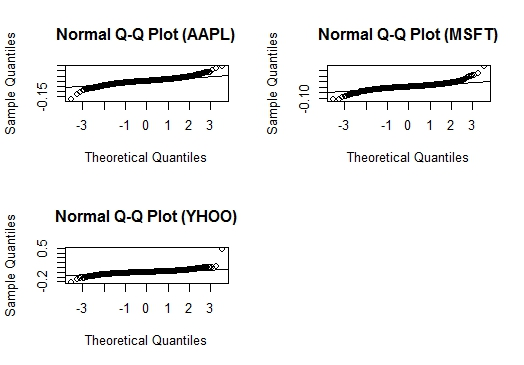
\includegraphics[width=1\linewidth]{Figuras/QQplot}
	\caption[Gráficos QQ]{Gráficos QQ plot.}
	\label{fig:qqplot}
\end{figure}
 
 Después, como se muestra en la gráfica \ref*{fig:histmarg}, si analizamos marginalmente el histograma empírico de los retornos de cada compañía podemos observar que la kurtosis parece ser mayor que el de una distribución normal, lo cual se puede verificar al calcular los momentos muestrales, pues para la empresa apple se tiene un coeficiente de kurtosis de $5.986$, para Microsoft de $10.397$ y para yahoo de $56.217$. También el sesgo muestral de cada compañía es de $-0.178$, $0.497$ y de $2.482$ respectivamente.  
 
 \begin{figure}[h]
 	\centering
 	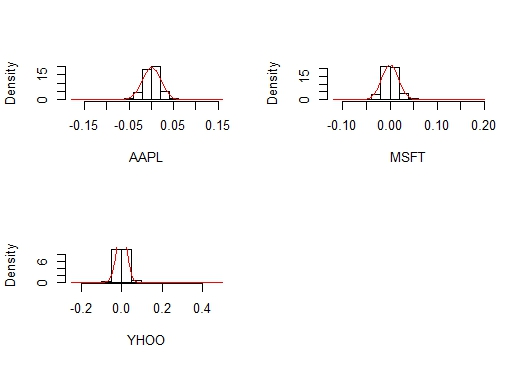
\includegraphics[width=1\linewidth]{Figuras/histmarg}
 	\caption{Histogramas}
 	\label{fig:histmarg}
 \end{figure}

Dicho lo anterior, tenemos evidencia para creer que marginalmente las distribuciones de los retornos de cada compañía no provienen de una distribución normal, lo cual podemos probar mediante la prueba Shapiro-Wilk del paquete $stats$ de $R$.

Implementando la prueba Shapiro-Wilk para cada conjunto de datos obtenemos que la estadística de prueba $w$ para Apple es de $0.94$, de $0.9065$ para Microsoft, y de $.8427$ para Yahoo; todas las pruebas tienen un valor $p$ de prácticamente cero, lo que rechaza la hipótesis de normalidad para los tres casos.

Una vez teniendo que las distribuciones marginales no provienen de una distribución normal, tenemos motivos para creer que la distribución conjunta de las tres compañías no es normal multivariada, pues de serlo sus distribuciones marginales debieran ser normales, lo cual se prueba a continuación.


Como se mencionó anteriormente, después de aplicarse la prueba de Marida, se obtuvo que el estadístico de prueba para el sesgo tiene un valor de $18.1$ , mientras que el de Kurtosis de $141.41$, ambos estadísticos mostraron un valor $p$ de cero, con lo cual se rechaza la hipótesis de que los datos provienen de una distribución normal multivarada.

Para la prueba Henz-Zirklers se obtuvo un estadística de prueba de 40.83, e igualmente un valor $p$ de cero con lo que igualmente se rechaza la hipótesis de que los datos fueron generados por una distribución normal multivariada. 

Por lo tanto, si juntamos los gráficos marginales y las pruebas realizadas, concluimos que el conjunto de datos no fue generado por una distribución normal multivariada.


\subsection{Código en R para la prueba de multinormalidad}

\lstinputlisting[language=R]{codigo/pruebas.r}

    

\end{document}




